%% Corrosion Science (Elsevier) -- CAS single-column template (cas-sc)
%% Companion version of the npj Materials Degradation submission
%% (paper/main-snjnl.tex).  Same science, same numbers; restructured to the
%% Elsevier order (Methods as section 2 rather than at the back) and
%% reformatted from sn-jnl to cas-sc.
%%
%% cas-sc is the single-column member of Elsevier's CAS bundle.  Being one
%% column, the figures keep the \textwidth sizing they have in the npj version
%% and no float needs promoting to a starred environment.
\documentclass[a4paper,fleqn]{cas-sc}

%% Corrosion Science numbers its references.  The CAS bundle ships only an
%% author-year .bst (cas-model2-names), so the numbered style comes from natbib.
\usepackage[numbers,sort&compress]{natbib}
\usepackage{amsmath,amssymb,amsfonts}
\usepackage{graphicx}
\usepackage{booktabs}
\usepackage{multirow}

%% Long unbreakable tokens (X6CrNiNb18-10) overrun the measure; let TeX stretch
%% a little rather than leave an overfull line.
\emergencystretch=1em

\graphicspath{{figures/}}

\begin{document}

\let\WriteBookmarks\relax
\def\floatpagepagefraction{1}
\def\textpagefraction{.001}

\shorttitle{Identifiability of a point defect model for AISI~347}
\shortauthors{C. G. Tetsassi Feugmo}

\title[mode=title]{Identifiability of a point defect model for oxide growth on AISI~347}

\author[1]{Conrard Giresse Tetsassi Feugmo}[orcid=0000-0002-8992-4335]
\cormark[1]
\ead{giresse.feugmo@gmail.com}

\address[1]{Department of Chemistry and Department of Physics \& Astronomy,
            University of Waterloo, 200 University Avenue West,
            Waterloo, ON N2L 3G1, Canada}

\cortext[1]{Corresponding author.}

\begin{abstract}
Mechanistic corrosion models are routinely fitted with four to six
parameters to a handful of measurements and then extrapolated across
service lifetimes, yet whether the data determine those parameters is
almost never tested. We identify a reduced point defect model for the
duplex oxide grown on Nb-stabilized AISI~347 (X6CrNiNb18-10) in
simulated boiling-water-reactor hydrothermal water
(240~$^\circ$C, 7~MPa, 0.4~ppm dissolved O$_2$) from published
depth-profile data at three exposure times, by differentiable
physics-informed inversion validated against an exact closed-form
reference. Profile likelihood, cross-checked against a 1000-member
bootstrap and a prior-relaxation test, leaves one of the five fitted
parameters undetermined and a second only weakly determined, while a
residual decomposition puts 95\% of the fit statistic on three chromium
points and 80\% on one. The kinetics fit the calibration data as well as
an empirical power law but extrapolate very differently: at ten years
the power law predicts a 3.5 to 6.3 times thicker barrier layer than the
mechanistic 535~nm (bootstrap 95\% interval 447--704~nm), a prediction
varying 1.19 to 1.56-fold across the scanned operating envelope. A
designed exposure beyond roughly 3000~hours would discriminate the two.
We further document and remedy a failure mode specific to sparse-data
inversion.
\end{abstract}

%% Corrosion Science classifies keywords: A. materials, B. techniques
%% and methods, C. processes and phenomena.
\begin{keywords}
A. Stainless steel \sep
B. Modelling studies \sep
C. Oxidation \sep
C. Passive films \sep
C. High temperature corrosion
\end{keywords}

\maketitle

\section{Introduction}\label{sec:intro}

Nb-stabilized austenitic stainless steel AISI~347 (X6CrNiNb18-10) is
used in boiling-water-reactor (BWR) internals and piping for its
resistance to weld-decay sensitization, yet the evolution of its passive
oxide film under reactor-representative hydrothermal water has so far
had no mechanistic predictive model. Current practice for predicting
oxide behavior on light-water-reactor internals relies either on
operational water-chemistry criteria framed around threshold
electrochemical corrosion potential (ECP) and dissolved-oxygen
levels~\citep{macdonald1992hwc,lin1996ecp,yeh1995damage1,yeh1996damage2},
which say nothing about oxide thickness or composition, or on
data-driven machine-learning models of crack-growth
rate~\citep{igscc_ml_uq2025}, which are equally silent on the underlying
oxide chemistry.

The duplex oxide that austenitic stainless steels develop in
high-temperature water---a Cr-rich inner spinel layer growing by
solid-state transport beneath an Fe-rich outer layer formed by
precipitation---is well established for the 304/316
grades~\citep{robertson1991mechanism,stellwag1998mechanism,ziemniak2002corrosion,kuang2010oxidation,terachi2008corrosion,kim1999oxide,lister1987release},
and the point defect model (PDM) of Chao, Lin, and
Macdonald~\citep{chao1981pdm1,lin1981pdm2,macdonald1992pdm,macdonald2011history},
in the tradition of high-field oxidation
theory~\citep{cabrera1949oxidation}, provides the standard mechanistic
description: vacancy-mediated transport under a high interfacial field,
yielding closed-form thickness-versus-time laws tied to interfacial
reaction kinetics. Li et al.~\citep{li2020scwpdm} extended this
framework to supercritical water. For AISI~347 specifically, Veile et
al.~\citep{veile2024} recently provided the first detailed
characterization of the duplex oxide developed in simulated BWR
hydrothermal water, resolving Cr-rich barrier and Fe-rich outer layers
by energy-dispersive X-ray (EDX) depth profiling at three exposure
times; their analysis stops at empirical per-element power-law fits,
with no shared physical parameter set connecting the layers and no
assessment of how far those fits can be extrapolated.

This paper adapts the supercritical-water PDM
formulation~\citep{li2020scwpdm} to the subcritical hydrothermal-water
regime and identifies its kinetics from the Veile et al.\ dataset with a
differentiable, physics-informed inversion framework. The alloy
specificity of the result lies in the data, not the model structure:
the reaction network contains nothing Nb-specific, and what is delivered
is the first PDM identification against the only depth-profile dataset
available for this alloy and environment. Beyond the identification, the
framework addresses a methodological gap that recurs across four decades
of PDM parameter estimation. Whether calibrated against electrochemical
impedance spectra~\citep{bojinov_mcm,ss316ln_pdm2024,ss321_pdm} or
against depth-profile data, four-to-six-parameter models are routinely
fit to three-to-six data points, and while parameter confidence
intervals and correlations are sometimes
reported~\citep{identifiability_electrochem1996}, we are not aware of a
formal profile-likelihood or bootstrap identifiability characterization
of a PDM fit. The distinction between ``the model fits'' and ``the data
constrain the parameters'' becomes consequential exactly when the fitted
model is meant to extrapolate beyond its calibration window, as here.
We close this gap with tools mature in adjacent
fields~\citep{raue2009identifiability,efron1979bootstrap,wieland2021identifiability},
standard in systems biology~\citep{biosystems_identifiability} and
increasingly applied to battery models~\citep{p2d_identifiability2021},
built directly into the inversion rather than bolted on afterward.

At the core of the framework is a physics-informed neural
solver~\citep{raissi2019pinn,karniadakis2021piml}, a neural
spectral-element method (NSEM). Kinetic parameters
are recovered by a hard-constrained inversion in which the trajectories
are generated by differentiable Runge--Kutta integration, so the
governing equations are satisfied exactly by construction; a classical
least-squares solver serves as an independent reference, and the two
agree to within 0.6\% on every parameter and to identical $\chi^2$. The
same machinery emulates the forward model with two neural backbones and,
in a soft-constrained joint field-and-parameter mode, extends to the
spatial transport problem.

It is worth stating at the outset what that machinery is, and is not,
doing here. The reduced kinetics admit a closed-form solution, and the
steady spatial problem admits both an analytic reference and a Newton
solve; classical methods therefore reproduce every result in this paper,
and in the spatial case do so more accurately. The neural solver is not
required by this problem, and we do not claim that it is. What the
application provides is the complementary thing---a real-data validation
of the framework against exact references, the conditions for which are
precisely the conditions under which the solver is dispensable---and,
out of that validation, a transferable negative result. Two further
distinctions matter. The property doing the statistical work is
\emph{differentiability} rather than the neural representation: exact
parameter gradients through a vectorized solver are what make profile
likelihood, a thousand-member bootstrap, prior-relaxation scans and a
dense operating-envelope grid affordable, and closed-form models with
automatic differentiation share that property. The neural representation
itself becomes necessary only where no closed form or cheap forward solve
exists---coupled potential and transport fields solved
self-consistently, moving-boundary inverse problems in which fields and
parameters are unknown together, or constitutive functions of unknown
form inferred from profile data---and the value of a validated,
failure-mode-characterized framework is realized there rather than here.
Our prior work demonstrated this machinery on the PDM
against synthetic benchmarked data, cataloguing four training-time
failure modes~\citep{farooqi2025pinnpdm}; the present paper is its first
application to real experimental data, and in carrying it out we document
and remedy a fifth failure mode specific to sparse-real-data inversion:
joint field-and-parameter training can settle into an equilibrium that
satisfies the data loss while leaving the governing equation only
approximately satisfied, exposed only by re-solving the recovered
parameters through an exact forward solve. Loss-balancing pathologies of
this general kind are a recognized theme in physics-informed
training~\citep{wang2022ntk,krishnapriyan2021failure}, and a
contemporaneous study reports a closely related diagnosis in an
unrelated domain~\citep{pinnverse2025}; the contribution here is its
documentation, its remedy, and a self-consistency check that travels
with the framework.

The remainder of the paper sets out the model and the inversion
methodology, and then the results: the reduced model and its
differentiable identification, the identifiability and uncertainty
analysis, the physics-informed inversion failure mode and its remedy, the
spatial extension and zero-parameter composition predictions, the nickel
enrichment zone, and the long-time predictions and operating-envelope
sensitivity. A discussion and conclusions follow.


\section{Model and methods}\label{sec:methods}

\subsection{Reduced-model derivation}\label{sec:model-methods}

The apparent-parameter system~\eqref{eq:odebl}--\eqref{eq:odeol}
summarized in Section~\ref{sec:model} is derived in full in the
Supplementary Information (Section~S1): the interfacial reaction
network, the constant-field potential distribution, the constant-volume
coupling that collapses the two growth rates into an affine
relationship, and the log-space-stabilized closed-form solutions. The
derivation also documents known errata in the source
formulations~\citep{li2020scwpdm}. The closed-form solutions of
Eqs.~\eqref{eq:odebl}--\eqref{eq:odeol} agree with Radau numerical
integration to better than $6\times10^{-11}$~nm (SI, Fig.~S1), and the
affine outer-layer form agrees with the closed form of
Ref.~\citep{li2020scwpdm} to better than $1\times10^{-10}$~nm.

\subsection{Experimental data}\label{sec:data}

Veile et al.~\citep{veile2024} exposed X6CrNiNb18-10 coupons to
simulated BWR hydrothermal water (240$^\circ$C, 7~MPa, 0.4~ppm dissolved
O$_2$) for 72, 168, and 480~h and measured element-resolved oxide layer
thicknesses by focused-ion-beam cross-sections with EDX line scans.
Table~\ref{tab:data}, given with the model ladder in
Section~\ref{sec:ladder}, reproduces the digitized layer-thickness means
used as the inversion target throughout this paper. The digitization
was checked against their own reported empirical fits: a scan-level
linear-space least-squares refit of $L = k\,t^n$ to our digitized
chromium data reproduces their published coefficients to four
significant figures ($k = 6.522$ versus their 6.521, $n = 0.4964$
versus 0.4964), which bounds the digitization error well below the
scan-to-scan scatter. For the iron layer the reported scan-to-scan
physical scatter of the discrete-crystal outer layer exceeds
digitization precision, so their reported layer means are used as the
authoritative data. No synthetic or simulated data enters the
kinetic identification; synthetic data appears only as an explicitly
labeled recovery test (Section~\ref{sec:pinn}).

\subsection{Statistical inversion and identifiability analysis}\label{sec:stats}

All fits minimize the weighted least-squares objective
\begin{equation}
\begin{split}
\Phi(\theta) = {}&
\sum_{i=1}^{3} \frac{\left[L_\text{bl}(t_i;\theta) - \bar{L}_{\text{Cr},i}\right]^2}{\sigma_{\text{Cr},i}^2}
+ \sum_{i=1}^{3} \frac{\left[L_\text{ol}(t_i;\theta) - \bar{L}_{\text{Fe},i}\right]^2}{\sigma_{\text{Fe},i}^2} \\
&+ \left(\frac{\ln L_0 - \ln 2\,\text{nm}}{0.60}\right)^{\!2},
\end{split}
\label{eq:objective}
\end{equation}
where $\bar{L}$ and $\sigma$ are the layer means and standard errors of
Table~\ref{tab:data} and the final term is a Gaussian prior in
log-parameter space on the initial barrier-layer thickness, centered on
the 1--5~nm air-formed film on high-Cr stainless steel. It is the only
prior in the objective, and it is carried because the exposure-time data
give $L_0$ no interior optimum at all: without it the estimate runs to
zero (Table~\ref{tab:priortest}). Earlier versions of this analysis also
placed a prior on $\mathrm{PBR}_\text{eff}$, centered on 1.05 and
described as the stoichiometric value. That center does not survive a
chromium mass balance (Section~\ref{sec:discussion}), so the prior has
been removed and $\mathrm{PBR}_\text{eff}$ is determined by the
likelihood alone throughout. The classical minimization
uses Levenberg--Marquardt least squares in log-parameter space (which
enforces positivity by construction), warm-started and verified against
grid restarts; convergence tolerances are $10^{-8}$. The equivalent
hard-mode physics-informed inversion (Section~\ref{sec:nsem}) minimizes
the same objective with the trajectories generated by differentiable
Runge--Kutta integration, and is the primary engine of this work; the
classical solver serves as an independent cross-check. Because the two
inversions agree to within 0.6\% on every parameter and to an identical
$\chi^2$, the deterministic parameter values and curves reported
throughout (Figs.~\ref{fig:fits}--\ref{fig:longtime}) are the converged
optimum common to both.

Profile-likelihood scans fix one parameter on a grid of $\pm1.5$
natural-log units about the optimum (61 points) and re-optimize all
others under the full objective~\eqref{eq:objective}; the
$\Delta\chi^2$ values reported are computed over the data residuals
alone, so a prior-dominated parameter is exposed as flat rather than
masked. The parametric bootstrap resamples each layer mean from a
Gaussian with its standard error (1000 members, all refits converged;
positivity is guaranteed by the log-space parametrization) and refits
the full objective.

Because two of the parameters are prior-dominated, the number of
data-determined parameters is between three and five, and the residual
degrees of freedom for the accepted five-parameter model are
correspondingly between 1 and 3 for the six data points. Goodness-of-fit
statements are therefore given for both endpoints of this
bracket rather than a single nominal degree-of-freedom count.

\subsection{Physics-informed spectral-element solver}\label{sec:nsem}

The physics-informed forward and inverse solves use spectral-element
networks built on discrete variational-representation collocation
operators, applied to the PDM family in our prior
work~\citep{farooqi2025pinnpdm}; we refer to the resulting neural
spectral-element-method solver as NSEM. Each field is represented by an
element network evaluated on a collocation node set, physical residuals
are enforced at the nodes through a first-integral or collocation
formulation, loss terms are combined by a balanced-residual dynamic
reweighting aggregator, and optimization proceeds in two phases (Adam,
then L-BFGS). Full architecture, loss definitions, and hyperparameters
for every configuration are tabulated in the SI (Section~S4).

The machinery is used in three configurations
(Fig.~\ref{fig:nsem_workflow}): a ``hard'' zero-dimensional inverse, in
which the kinetic parameters are the only learnable quantities and the
trajectories are generated by differentiable Runge--Kutta integration,
so Eqs.~\eqref{eq:odebl}--\eqref{eq:odeol} are satisfied exactly by
construction; a ``soft'' zero-dimensional inverse, in which field
networks represent the trajectories directly and are trained jointly
with the parameters against a combined data-and-physics loss (the
configuration in which the failure mode of Section~\ref{sec:pinn} is
exposed); and the spatial extension of Section~\ref{sec:spatial}, where
no differentiable-integrator shortcut exists and the soft-mode field
representation is the only option, verified against an independent
Newton solve on the same node set.

Every configuration is checked against an independent reference before
its results are used. The classical baseline itself is established
to machine precision (Section~\ref{sec:model-methods}). Two
neural backbones---a multilayer perceptron (MLP) and a
Kolmogorov--Arnold network (KAN)~\citep{liu2024kan}---are evaluated in
the same harness to test backbone sensitivity, both to the same
acceptance criterion (relative $L^\infty$ error $\le0.5\%$ against the
closed form). All results are backed by an automated test suite (25
tests) checking parity between closed-form, Newton, and neural
solutions; the suite ships with the code release (see Data and code
availability).

\begin{figure}[htbp]
\centering
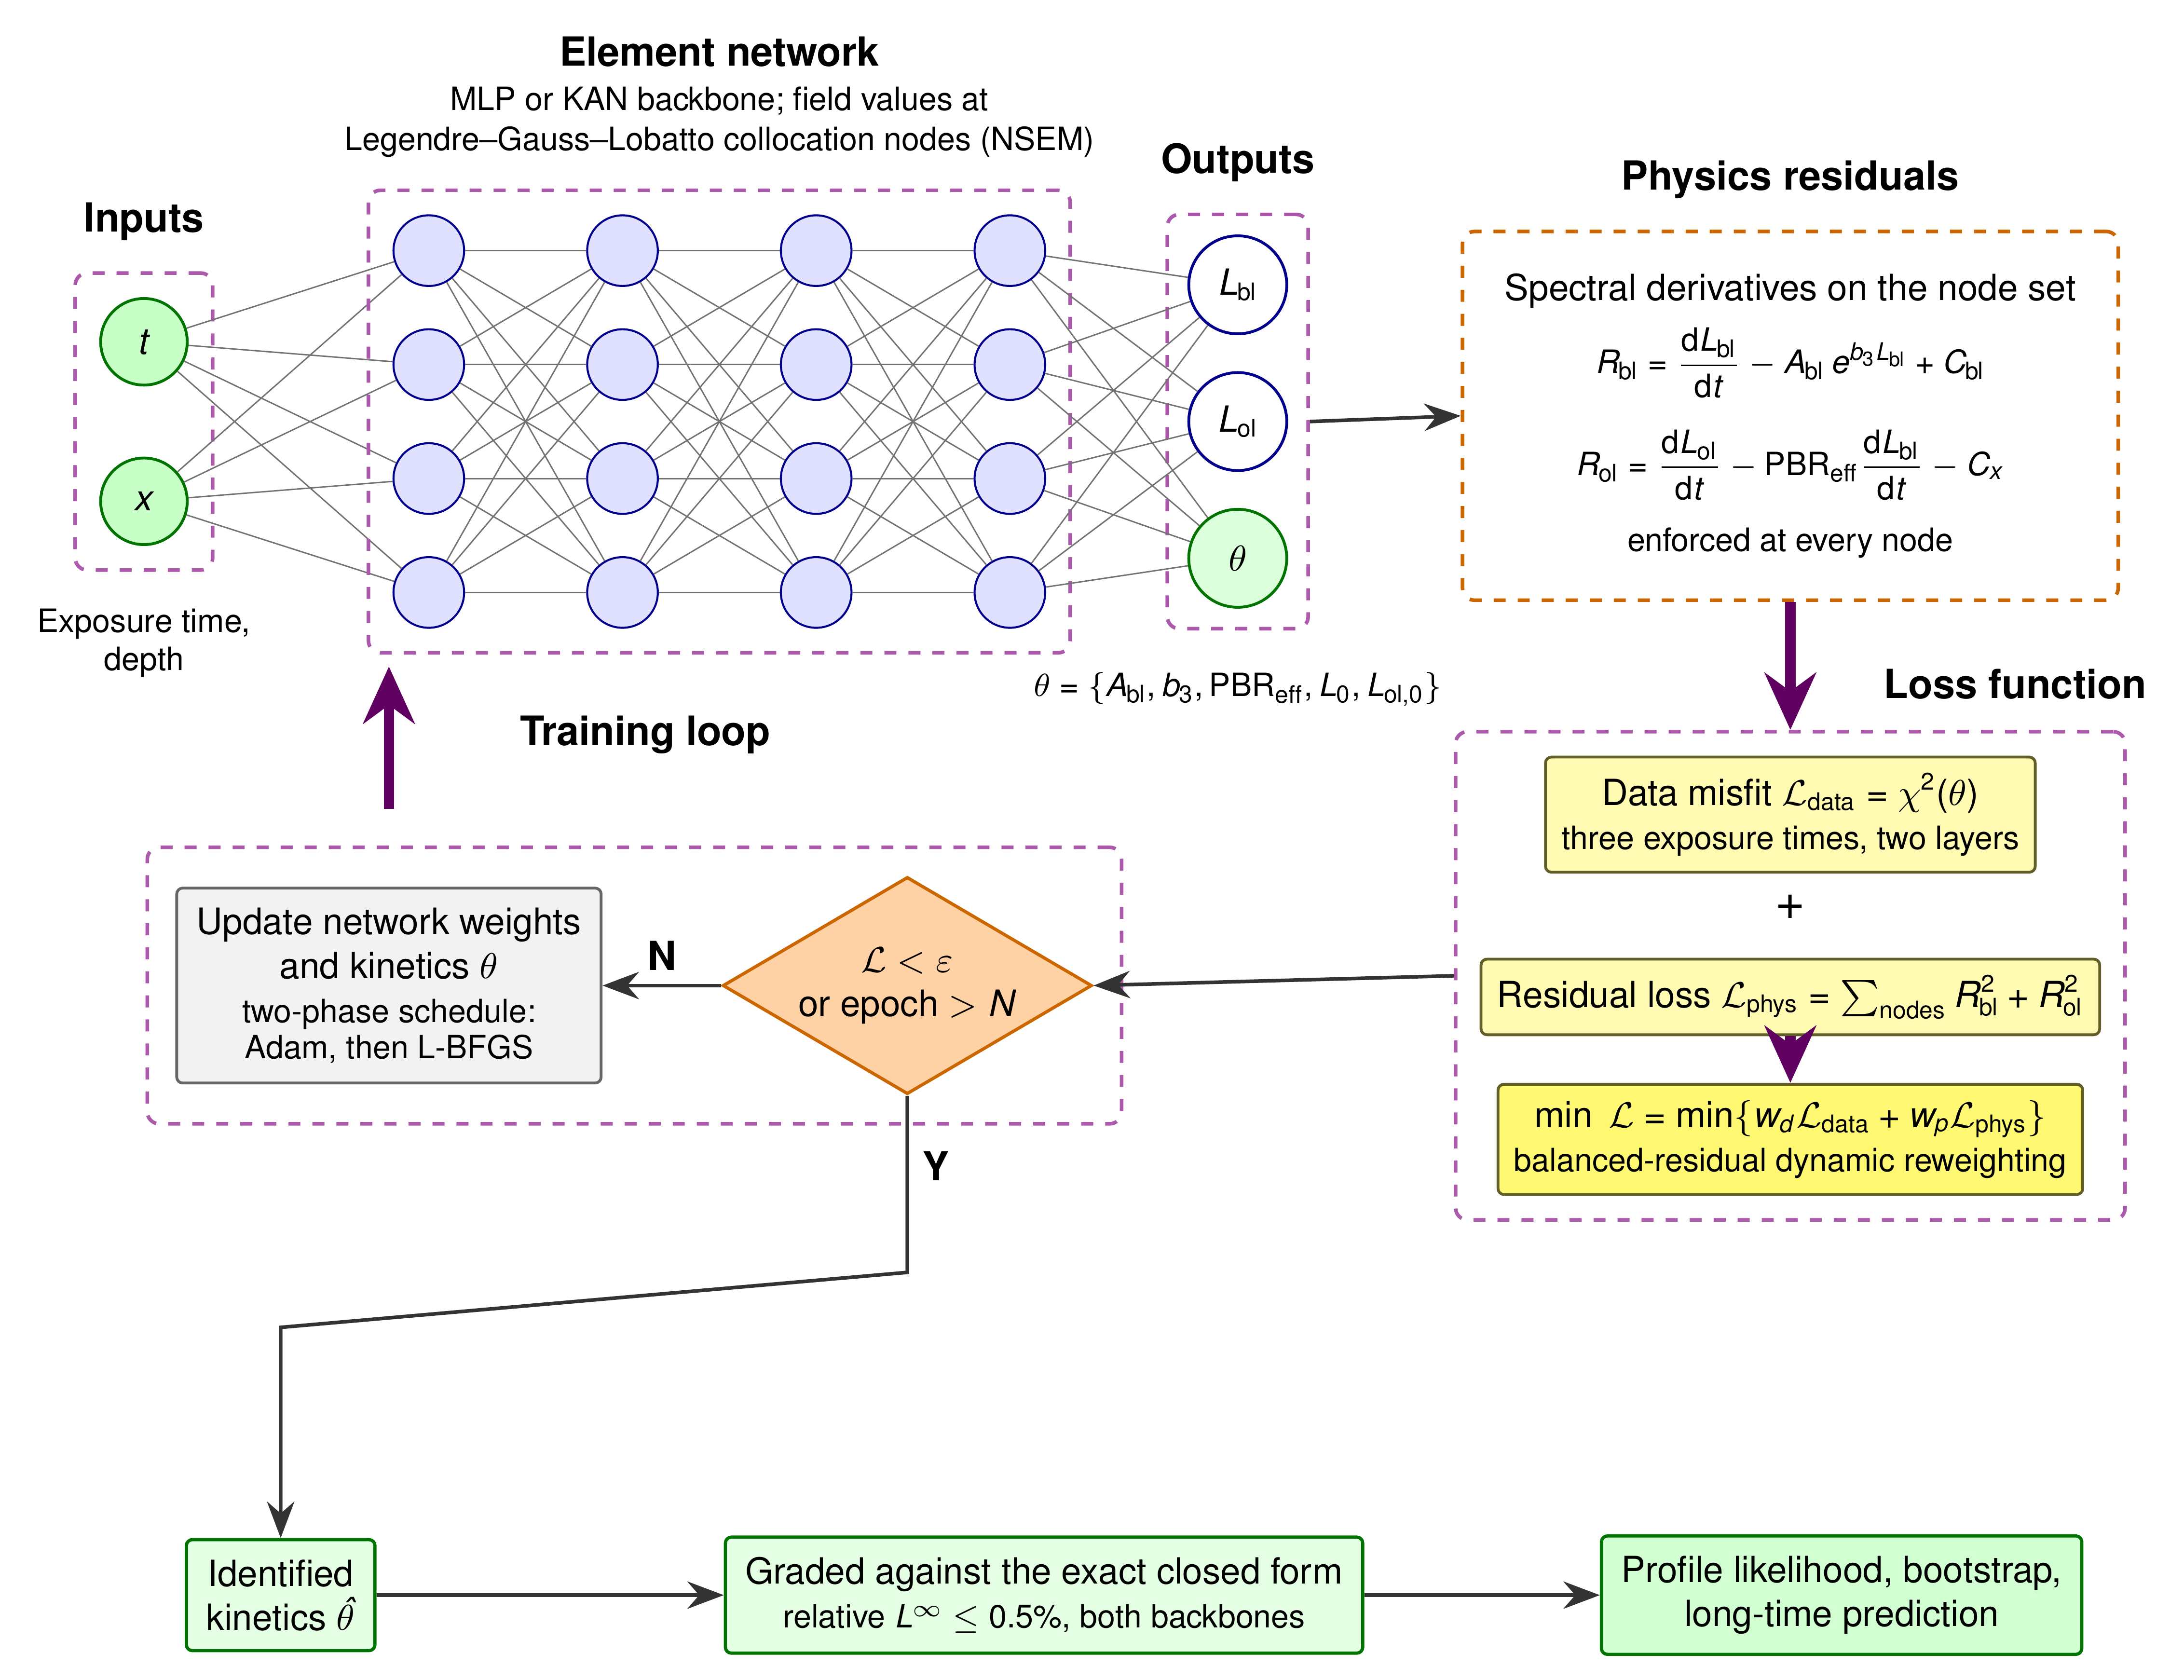
\includegraphics[width=\textwidth]{figures/fig_nsem_workflow.png}
\caption{NSEM workflow. (a) Shared representation: field values on a
discrete-variational-representation collocation node set produced by an
element network (MLP or KAN backbone), with physics residuals enforced
at every node. (b) The three configurations used in this work, the
shared two-phase optimization, and the verification step each
configuration passes before its results are reported.}
\label{fig:nsem_workflow}
\end{figure}



\section{Results}\label{sec:results}

\subsection{The reduced point defect model}\label{sec:model}

The governing kinetics follow the PDM in the formulation Li et
al.~\citep{li2020scwpdm} developed for supercritical water,
adapted here to subcritical hydrothermal-water conditions. The oxide
Veile et al.~\citep{veile2024} characterize on X6CrNiNb18-10 is a
duplex scale (Fig.~\ref{fig:schematic}): a chromium-rich,
nanocrystalline spinel barrier layer growing into the metal, and
discrete iron-rich magnetite crystals forming a porous outer layer, with
a nickel enrichment zone at the receding metal/barrier-layer interface.
The base kinetics treat the nickel zone as an inert consistency check; a
dedicated transport model for it is developed in
Section~\ref{sec:nickel}. The full reaction network,
potential-distribution assumptions, and rate-law derivation are given in
the Supplementary Information (SI, Section~S1, which also documents
known errata in the source papers), with numerical validation in
Section~\ref{sec:model-methods}; here we state the structure that
determines the apparent-parameter system actually fit.

Two classes of interfacial reaction move the model's interfaces:
barrier-layer growth into the metal, driven by oxygen-vacancy generation
at the metal/barrier-layer interface, and barrier- and outer-layer
destruction by chemical conversion and dissolution. Every rate constant
depends on the applied potential and local pH, and the growth reaction
additionally on the barrier-layer thickness through an exponential term
whose sign is fixed by the PDM's constant-field assumption: growth
decelerates exponentially as the film thickens, producing
logarithmic-to-parabolic kinetics and, for nonzero dissolution, an
eventual finite steady-state thickness. Because the open-circuit
potential and pH are constant over a given exposure (the water is
neutral, unbuffered, and of very low conductivity; at 240$^\circ$C the
neutral pH is approximately 5.6), they cannot be separated from the
growth reaction's intrinsic rate constant using thickness-versus-time
data alone. The potential and pH dependence is therefore absorbed into
a single apparent growth prefactor, and the film-thickness dependence
into a single apparent field-related exponent; it is these apparent
parameters, not the underlying elementary rate constants, that the
identification recovers.

The outer layer's growth is coupled to the barrier layer's through a
constant-volume constraint: metal consumption at the receding
metal/barrier-layer interface and barrier-layer advance proceed at the
same rate, which, for negligible barrier-layer destruction in this
ultrapure-water environment, collapses the two growth rates into an
exact affine relationship. This reduction is algebraically simpler than
the closed form of Ref.~\citep{li2020scwpdm} and the two forms agree to
better than $1\times10^{-10}$~nm. The resulting apparent system is
\begin{align}
\frac{\mathrm{d}L_\text{bl}}{\mathrm{d}t} &=
A_\text{bl}\, e^{\,b_3 L_\text{bl}} - C_\text{bl},
\label{eq:odebl}\\
\frac{\mathrm{d}L_\text{ol}}{\mathrm{d}t} &=
\mathrm{PBR}_\text{eff}\,
\frac{\mathrm{d}L_\text{bl}}{\mathrm{d}t} - C_x,
\label{eq:odeol}
\end{align}
where $L_\text{bl}$ and $L_\text{ol}$ are the barrier- and outer-layer
thicknesses, $A_\text{bl}$ (nm\,h$^{-1}$) is the apparent growth
prefactor, $b_3<0$ (nm$^{-1}$) the apparent field-related exponent,
$C_\text{bl}\ge0$ (nm\,h$^{-1}$) the barrier-layer dissolution rate,
$\mathrm{PBR}_\text{eff}$ the apparent (Pilling--Bedworth-type)
outer-to-barrier growth-rate ratio, and $C_x$ (nm\,h$^{-1}$) a small
outer-layer dissolution term; the initial conditions
$L_\text{bl}(0)=L_0$ and $L_\text{ol}(0)=L_\text{ol,0}$ complete the
seven-parameter set. The system has closed-form solutions, stabilized in
log space so they remain numerically exact in both time limits (SI,
Section~S1.6). The field-related exponent maps to a field strength
through $b_3 = -\alpha_3\chi\gamma\varepsilon_f$, with $\alpha_3$ the
growth-reaction transfer coefficient, $\chi=8/3$ the spinel-averaged
cation charge, and $\gamma = F/RT = 22.6$~V$^{-1}$ at 240$^\circ$C; the
sensitivity of the derived $\varepsilon_f$ to the assumed $\alpha_3$ is
addressed in Section~\ref{sec:discussion}.

\begin{figure}[htbp]
\centering

\includegraphics[width=0.9\textwidth]{figures/fig1_model_schematic.png}
\caption{Duplex-oxide model schematic. (a) Layer structure (metal
$\vert$ Ni enrichment zone $\vert$ Cr-rich nanocrystalline spinel
barrier layer $\vert$ Fe-rich outer-layer crystals $\vert$ hydrothermal
water) and the retained interfacial reactions. (b) Potential
distribution across the duplex oxide under the constant-field
assumption. Reaction labels and potential-drop symbols follow the SI
derivation.}
\label{fig:schematic}
\end{figure}

\subsection{Differentiable inversion and the model ladder}\label{sec:ladder}

We identify the reduced kinetics by minimizing a weighted least-squares
objective (Section~\ref{sec:stats}, Eq.~\eqref{eq:objective}), solving
the inverse problem two independent ways: a hard-constrained
physics-informed neural inversion, in which the trajectories are produced
by differentiable Runge--Kutta integration so that
Eqs.~\eqref{eq:odebl}--\eqref{eq:odeol} hold exactly, and a classical
Levenberg--Marquardt solver. The two agree to within 0.6\% on every
parameter and to identical $\chi^2$ (Section~\ref{sec:pinn}); we
therefore report a single identified parameter set and use the ladder
below only to decide model structure.

We fit the reduced system~\eqref{eq:odebl}--\eqref{eq:odeol} to the
joint Cr and Fe thickness means (Table~\ref{tab:data}) in a nested model
ladder
(Table~\ref{tab:ladder}), each variant adding degrees of freedom to
test whether the flexibility is supported by the data. The
four-parameter core model (M1, $C_\text{bl}=C_x=0$,
$L_\text{ol,0}=0$) reaches $\chi^2 = 7.15$ only by driving
$\mathrm{PBR}_\text{eff}$ to 2.43, and still cannot reproduce the
disproportionately thick early iron layer under strict constant-volume
coupling from zero initial thickness; adding a free dissolution rate
(M2) does not help, because the fit drives that rate to zero. Releasing
the coupling entirely in the six-parameter M3 variant does not produce a
better model but a degenerate one, and with no prior to hold it back the
degeneracy is now the interior optimum rather than something a profile
has to expose: the growth prefactor and dissolution rate diverge
together to $\sim\!10^{3}$~nm\,h$^{-1}$ while the field parameter
collapses by four orders of magnitude to
$-4.4\times10^{-6}$~nm$^{-1}$, buying the lowest data $\chi^2$ in the
ladder (4.11) through an unphysical linear-growth escape route. Its
ten-year barrier-layer prediction is 155~nm against M4's 535~nm, so the
$\chi^2$ ordering and the physical ordering disagree outright. That M3
wins on fit and loses on physics is the clearest statement in this paper
of why $\chi^2$ cannot by itself select a model on six data points.
Parameter correlations of this kind have long been discussed
qualitatively in PDM fitting; the explicit demonstration of the full
ridge, its escape direction, and its capture of the unconstrained
optimum on real PDM data is, to our knowledge, new.

The trap is resolved by a single additional parameter, the initial
outer-layer thickness (M4): a nonzero starting population of Fe-rich
outer-layer crystals captures the rapid initial precipitation Veile et
al.\ observe by 72~h. This five-parameter model reduces the data
$\chi^2$ from 7.15 (M1) to 5.79, and does so while returning
$\mathrm{PBR}_\text{eff}$ to order unity, where M1 needed 2.43 to
compensate for the missing initial precipitate population. The six-parameter M5, which adds a
free dissolution rate on top of M4, reaches the same $\chi^2$ with that
rate indistinguishable from zero; it is carried forward only as the
alternative long-time branch it implies (finite saturation instead of
unbounded logarithmic growth, Section~\ref{sec:predictions}), not as a
competing fit. For M3 and M5 the free-parameter count equals the six
data points and the residual degrees of freedom are zero; their $\chi^2$
is nonetheless nonzero because the objective~\eqref{eq:objective} carries
one prior residual in addition to the six data residuals, so the fit is
not free to interpolate. No goodness-of-fit statistic is quoted for those
rows.

\begin{table}[htbp]
\centering
\caption{Layer-thickness data of Veile et al.~\citep{veile2024} (their
Fig.~9) used in this work: mean $\pm$ population standard deviation
over $n$ EDX line scans. The fits use standard errors
$\sigma = \mathrm{SD}/\sqrt{n}$. The Ni enrichment zone is not a
growing PDM layer and enters only the analysis of
Section~\ref{sec:nickel}.}
\label{tab:data}
\small
\begin{tabular}{lcccc}
\toprule
Layer & $t$ (h) & mean (nm) & SD (nm) & $n$ \\
\midrule
Cr (barrier) & 72 & 37.3 & 7.7 & 3 \\
 & 168 & 98.3 & 21.7 & 4 \\
 & 480 & 134.3 & 5.4 & 3 \\
Fe (outer) & 72 & 143.3 & 111.5 & 3 \\
 & 168 & 225.5 & 142.7 & 4 \\
 & 480 & 240.3 & 172.5 & 3 \\
Ni (zone) & 72 & 31.3 & 3.4 & 3 \\
 & 168 & 43.0 & 11.1 & 4 \\
 & 480 & 36.0 & 5.0 & 3 \\
\bottomrule
\end{tabular}
\end{table}

\begin{table}[htbp]
\centering
\caption{Model ladder: nested apparent-parameter models fit to the
joint Cr+Fe layer-thickness data. The M3 row is the interior optimum
reached from the standard starting point, and it sits on the degenerate
ridge itself: the growth prefactor and dissolution rate diverge together
to $\sim\!10^{3}$~nm\,h$^{-1}$ while the field parameter collapses to
$-4.4\times10^{-6}$~nm$^{-1}$. It attains the lowest data $\chi^2$ in
the ladder and the least defensible physics, predicting 155~nm at ten
years against M4's 535~nm; it is listed for completeness and rejected on
structure, not on fit.
The power law appears twice: evaluated at Veile et al.'s published
scan-level coefficients, and refit under the same weighted
objective~\eqref{eq:objective} as the mechanistic models. For M3 and
M5, $n_\text{free}$ equals the number of data points and dof $=0$.
$^\ddagger$The published-coefficient power law is \emph{evaluated}, not
fitted, against these six means---its coefficients were determined
elsewhere, on individual scans in unweighted linear space---so it costs
no degrees of freedom here and its residual dof is 6. No information
criterion is computed for that row.}
\label{tab:ladder}
\small
\begin{tabular}{lccccc}
\toprule
Model & Extra params & $n_\text{free}$ & $\chi^2_\text{data}$ & dof & $A_\text{bl}$ (nm/h) \\
\midrule
M1 core & --- & 4 & 7.15 & 2 & 0.7516 \\
M2 & $+C_\text{bl}$ & 5 & 7.15 & 1 & 0.7516 \\
M3 (degenerate) & $+C_\text{bl}, +C_x$ & 6 & 4.11 & 0 & 955.8 \\
\textbf{M4 (accepted)} & $+L_\text{ol,0}$ & 5 & \textbf{5.79} & 1 & \textbf{0.7269} \\
M5 & $+L_\text{ol,0}, +C_\text{bl}$ & 6 & 5.79 & 0 & 0.7269 \\
Power law (published coeffs) & $k,n$ per layer & 0$^\ddagger$ & 20.10 & 6$^\ddagger$ & --- \\
Power law (weighted refit) & $k,n$ per layer & 4 & 7.84 & 2 & --- \\
\bottomrule
\end{tabular}
\end{table}

The comparison with the empirical power law is reported both ways.
Evaluated at Veile et al.'s published per-layer coefficients the power
law gives $\chi^2 = 20.10$ against the joint layer means, but those
coefficients were fit to individual scans in unweighted linear space;
refit under the weighted objective~\eqref{eq:objective} it reaches
$\chi^2 = 7.84$ with four free parameters. On information criteria the
two descriptions are then statistically indistinguishable on this
dataset (Akaike criterion 15.8 for both; Bayesian criterion 14.8
mechanistic versus 15.0 power law; the small-sample-corrected criterion
is undefined for M4 at $n=6$, $n-k-1=0$, and is 55.8 for the power
law). These criteria are quoted as indicative only at this sample size.
The mechanistic model's advantage on the calibration window is not fit
quality---no comparison on three exposure times could demonstrate
that---but the physical coupling it enforces: the constant-volume
constraint ties the two layers through a single
growth-and-precipitation picture, where the power law treats each layer
as an independent curve (Fig.~\ref{fig:fits}); it is this coupling that
drives the divergent extrapolations of
Section~\ref{sec:predictions}.

On absolute goodness of fit, $\chi^2 = 5.79$ corresponds to $p = 0.016$
at one residual degree of freedom and $p \approx 0.12$ at three (the
effective-dof bracket of Section~\ref{sec:stats}). If the mild misfit
is real, the reported standard errors of the layer means understate the
scan-to-scan variability---consistent with the physical heterogeneity
Veile et al.\ report---and an error-scale correction of
$s = \sqrt{\chi^2/\text{dof}} = 1.4$--$2.4$ would widen every
uncertainty interval below by that factor. Unscaled intervals are
quoted throughout; no identifiability verdict changes under the maximal
scaling (the sharply identifiable parameters remain so at $2.4\times$
wider intervals, and the unidentifiable ones cannot get worse), but the
implications for the extrapolation bands are stated explicitly in
Section~\ref{sec:predictions}.

The recovered kinetics place the apparent growth prefactor at
$A_\text{bl} = 0.727$~nm/h and the field exponent at
$b_3 = -0.0125$~nm$^{-1}$ ($-1.25\times10^{5}$~cm$^{-1}$). The
recovered $\mathrm{PBR}_\text{eff} = 1.096$ carries no prior and is
therefore a statement of the likelihood alone. It sits near unity, and
roughly a factor of two below the value a chromium mass balance on this
alloy implies for an FeCr$_2$O$_4$ barrier. That comparison does not
survive scrutiny in either direction---the mass-balance figure is
phase-dependent, and the fitted parameter is not the same quantity once
outer-layer loss is admitted---and is taken up in
Section~\ref{sec:discussion}.

\subsubsection*{Where the fit statistic comes from}

A five-parameter model fitted to six means invites the question of which
data points actually carry the fit. Decomposing $\chi^2$ at the M4
optimum answers it (Fig.~\ref{fig:fits}e,f;
Table~\ref{tab:leverage}). The three chromium points contribute 95\% of
$\chi^2 = 5.79$ and the three iron points only 5\%: the outer layer's
scan-to-scan scatter is so large (standard errors of the mean of 32--45\%
of the mean, against 2--12\% for chromium) that it constrains the fit
only weakly. Within the chromium set the misfit is concentrated in a
single datum---the 168~h point, at $-2.15\sigma$, supplies 80\% of the
total---and the residual signs run $+$, $-$, $+$ across the three
exposures, a systematic pattern rather than scatter, indicating that the
\emph{curvature} of the fitted logarithmic law does not track the three
measured chromium thicknesses.

Two consequences follow, and both are carried through the rest of the
paper. First, the curvature parameter $b_3$ is what governs the long-time
extrapolation of Section~\ref{sec:predictions}, so a systematic curvature
residual on the only three points that constrain it is the dominant
structural caveat on the ten-year number---larger, in our view, than the
parametric uncertainty the bootstrap propagates. Second, the
constant-volume coupling and the initial-precipitate parameter
$L_\text{ol,0}$, although motivated by the iron layer, are in practice
constrained by it only weakly; the mechanistic reading of the iron
exponent in Section~\ref{sec:discussion} should be weighed accordingly.
Neither observation is grounds for preferring the power law, whose own
free parameters are fitted against the same six means with the same
leverage imbalance, but both bound how much any description calibrated on
this dataset can claim.

\begin{table}[htbp]
\centering
\caption{Residual and $\chi^2$ leverage decomposition of the accepted M4
fit. $\sigma$ is the standard error of the layer mean
(Table~\ref{tab:data}). The chromium layer carries 95\% of $\chi^2$ and
the 168~h chromium point alone carries 80\%.}
\label{tab:leverage}
\small
\begin{tabular}{lcccrr}
\toprule
Layer & $t$ (h) & $\sigma$ (nm) & Model (nm) & Residual ($\sigma$) & \% of $\chi^2$ \\
\midrule
Cr (barrier) & 72 & 4.45 & 41.4 & $+0.92$ & 14.7 \\
 & 168 & 10.82 & 74.9 & $-2.15$ & 80.1 \\
 & 480 & 3.14 & 134.8 & $+0.15$ & 0.4 \\
Fe (outer) & 72 & 64.37 & 158.9 & $+0.24$ & 1.0 \\
 & 168 & 71.35 & 195.6 & $-0.42$ & 3.0 \\
 & 480 & 99.59 & 261.2 & $+0.21$ & 0.8 \\
\midrule
\multicolumn{4}{l}{Total $\chi^2 = 5.79$} & Cr 5.51 & 95.2 \\
\multicolumn{4}{l}{} & Fe 0.28 & 4.8 \\
\bottomrule
\end{tabular}
\end{table}

\begin{figure}[htbp]
\centering
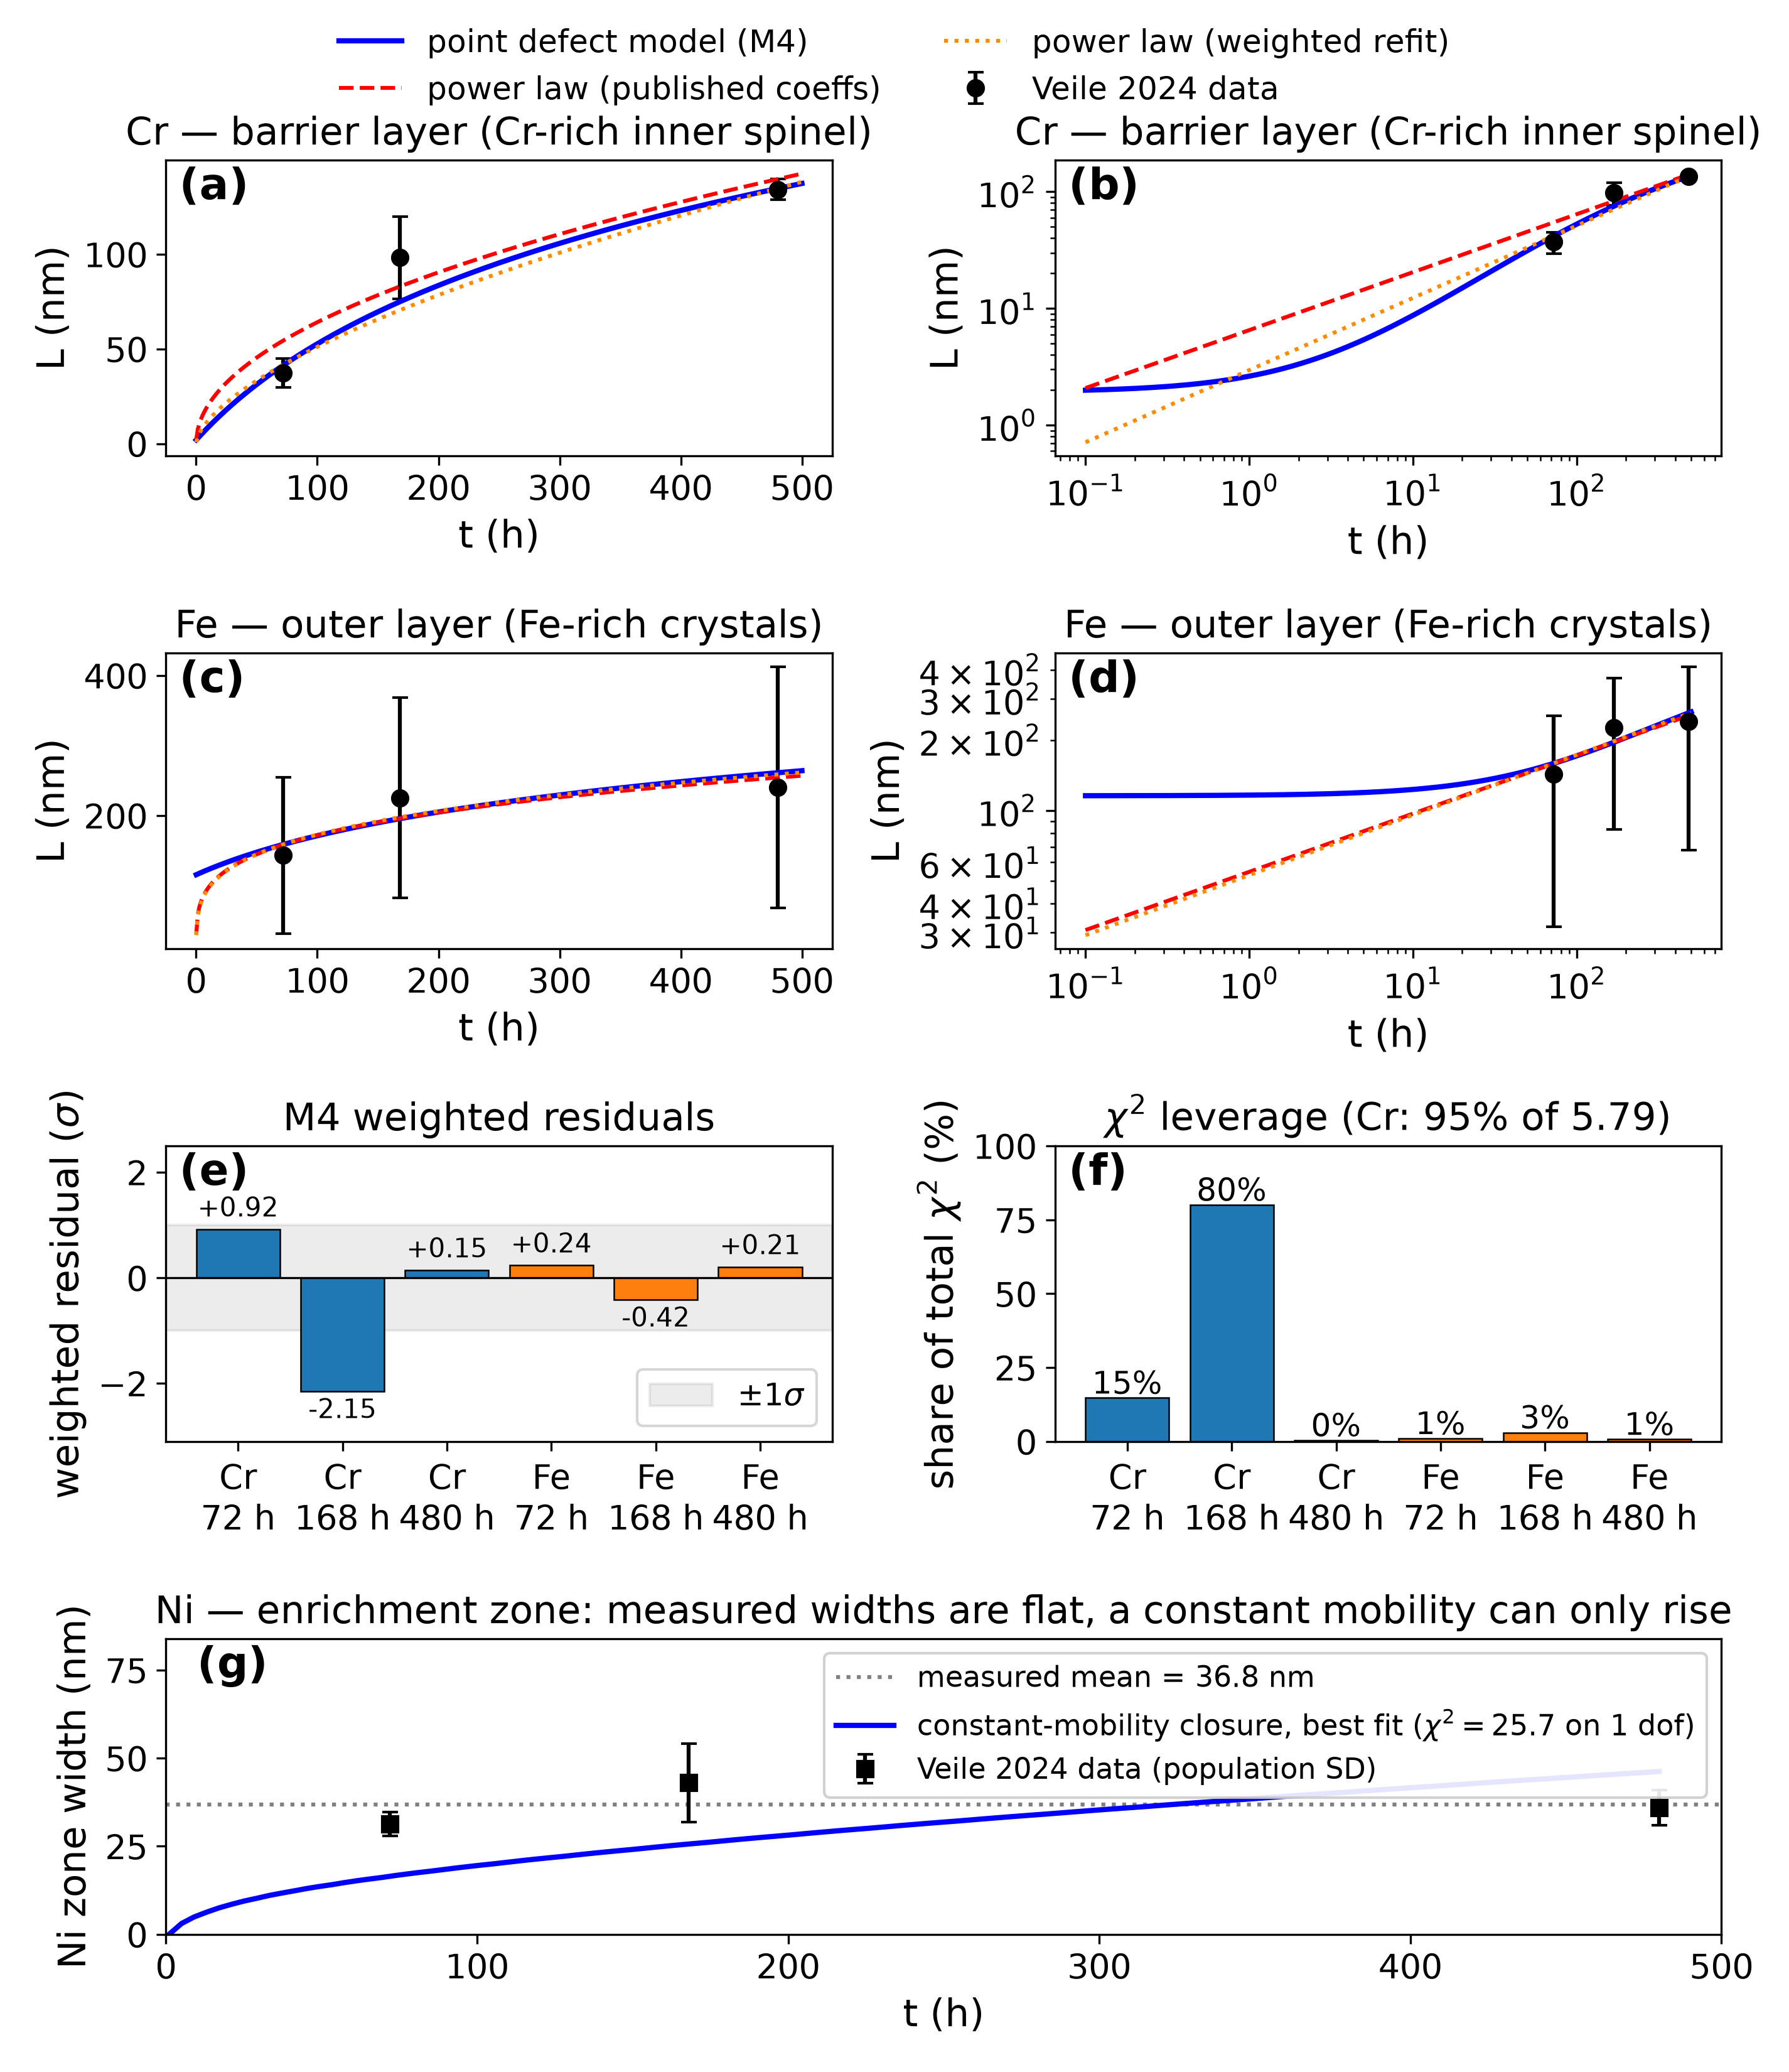
\includegraphics[width=\textwidth]{figures/fig3_fits_vs_data.png}
\caption{M4 fit and the empirical power law against the measured
layer-thickness data. (a, b)~Cr barrier layer, linear and log--log
axes; (c, d)~Fe outer layer, linear and log--log axes. Points with
error bars are the means $\pm$ standard deviations of
Table~\ref{tab:data} (the fits weight residuals by standard errors,
$\mathrm{SD}/\sqrt{n}$); curves are the M4 mechanistic fit and the two
power-law variants (published coefficients and weighted refit).
(e)~Weighted residuals of the M4 fit at the six data points, and
(f)~each point's share of the total $\chi^2$: the chromium layer carries
95\% of the fit statistic and the 168~h chromium point alone 80\%, with
the $+$, $-$, $+$ chromium residual pattern indicating a systematic
curvature miss rather than scatter (Table~\ref{tab:leverage}). (g)~Ni enrichment-zone
thickness, shown for completeness with its measured mean (dotted); as
in Veile et al.'s own analysis, this zone is not a growing PDM layer,
and its dedicated transport fit appears in Section~\ref{sec:nickel}.}
\label{fig:fits}
\end{figure}

\subsection{Parameter identifiability and uncertainty quantification}\label{sec:identifiability}

Profile-likelihood scans referenced to the joint global minimum
(Fig.~\ref{fig:profile}, Table~\ref{tab:params}) show that the three
exposure times sharply constrain three of the five M4 parameters: the
growth prefactor, field exponent, and initial outer-layer thickness
(maximum $\Delta\chi^2$ of 50, 130, and 58 across their scans). The
Pilling--Bedworth ratio is only weakly identifiable (maximum
$\Delta\chi^2$ 19.5, interval spanning an order of magnitude), and the
initial barrier-layer thickness is formally unidentifiable from the
exposure-time data (maximum $\Delta\chi^2$ of 1.0; its quoted interval
simply reflects the $\pm1.5$ natural-log scan range: the
parameter is unbounded within the scanned range and is set by the
air-film prior). A shallow secondary structure in the growth-prefactor
profile at low parameter values is a local optimum of the compensating
parameters; it sits more than six $\Delta\chi^2$ units above the global
minimum and does not affect the quoted interval. Separately, an
explicit search for a dissolution-rate upper bound from the thickness
data finds no bound below 1~nm/h: the model's two qualitatively
different long-time behaviors remain numerically indistinguishable
within the exposure window, a point taken up in
Section~\ref{sec:predictions}.

\begin{table}[htbp]
\centering
\caption{M4 parameters: fitted value, profile-likelihood 1$\sigma$
interval, 1000-member bootstrap mean $\pm$ standard deviation, and
identifiability verdict. The derived field strength is
$\varepsilon_f = 1.7\times10^4$~V/cm at the reference transfer
coefficient $\alpha_3 = 0.12$; its dominant (systematic) uncertainty is
the assumed $\alpha_3$, discussed in Section~\ref{sec:discussion}.
$^\dagger$For $L_0$ the bracket gives the scan-range endpoints, not
$\Delta\chi^2 = 1$ crossings: the profile never exceeds
$\Delta\chi^2 = 1$ anywhere in the scanned range. No parameter carries a
prior except $L_0$; $\mathrm{PBR}_\text{eff}$ is determined by the
likelihood alone.}
\label{tab:params}
\footnotesize
\setlength{\tabcolsep}{4pt}
\small
\begin{tabular}{lccccl}
\toprule
Parameter & Unit & M4 fit & Profile 1$\sigma$ & Bootstrap & Verdict \\
\midrule
$A_\text{bl}$ & nm/h & 0.7269 & [0.626, 0.845] & $0.735 \pm 0.122$ & identifiable \\
$b_3$ & nm$^{-1}$ & $-0.01249$ & [$-0.0145$, $-0.0108$] & $-0.01243 \pm 0.00202$ & identifiable \\
$\text{PBR}_\text{eff}$ & --- & 1.096 & [0.245, 2.32] & $1.169 \pm 0.931$ & weakly identifiable \\
$L_0$ & nm & 1.9237 & [0.429, 8.20]$^\dagger$ & $1.923 \pm 0.0358$ & not identifiable (prior-set) \\
$L_\text{ol,0}$ & nm & 115.58 & [25.79, 210.6] & $110.5 \pm 74.7$ & identifiable \\
\bottomrule
\end{tabular}
\end{table}

\begin{figure}[htbp]
\centering
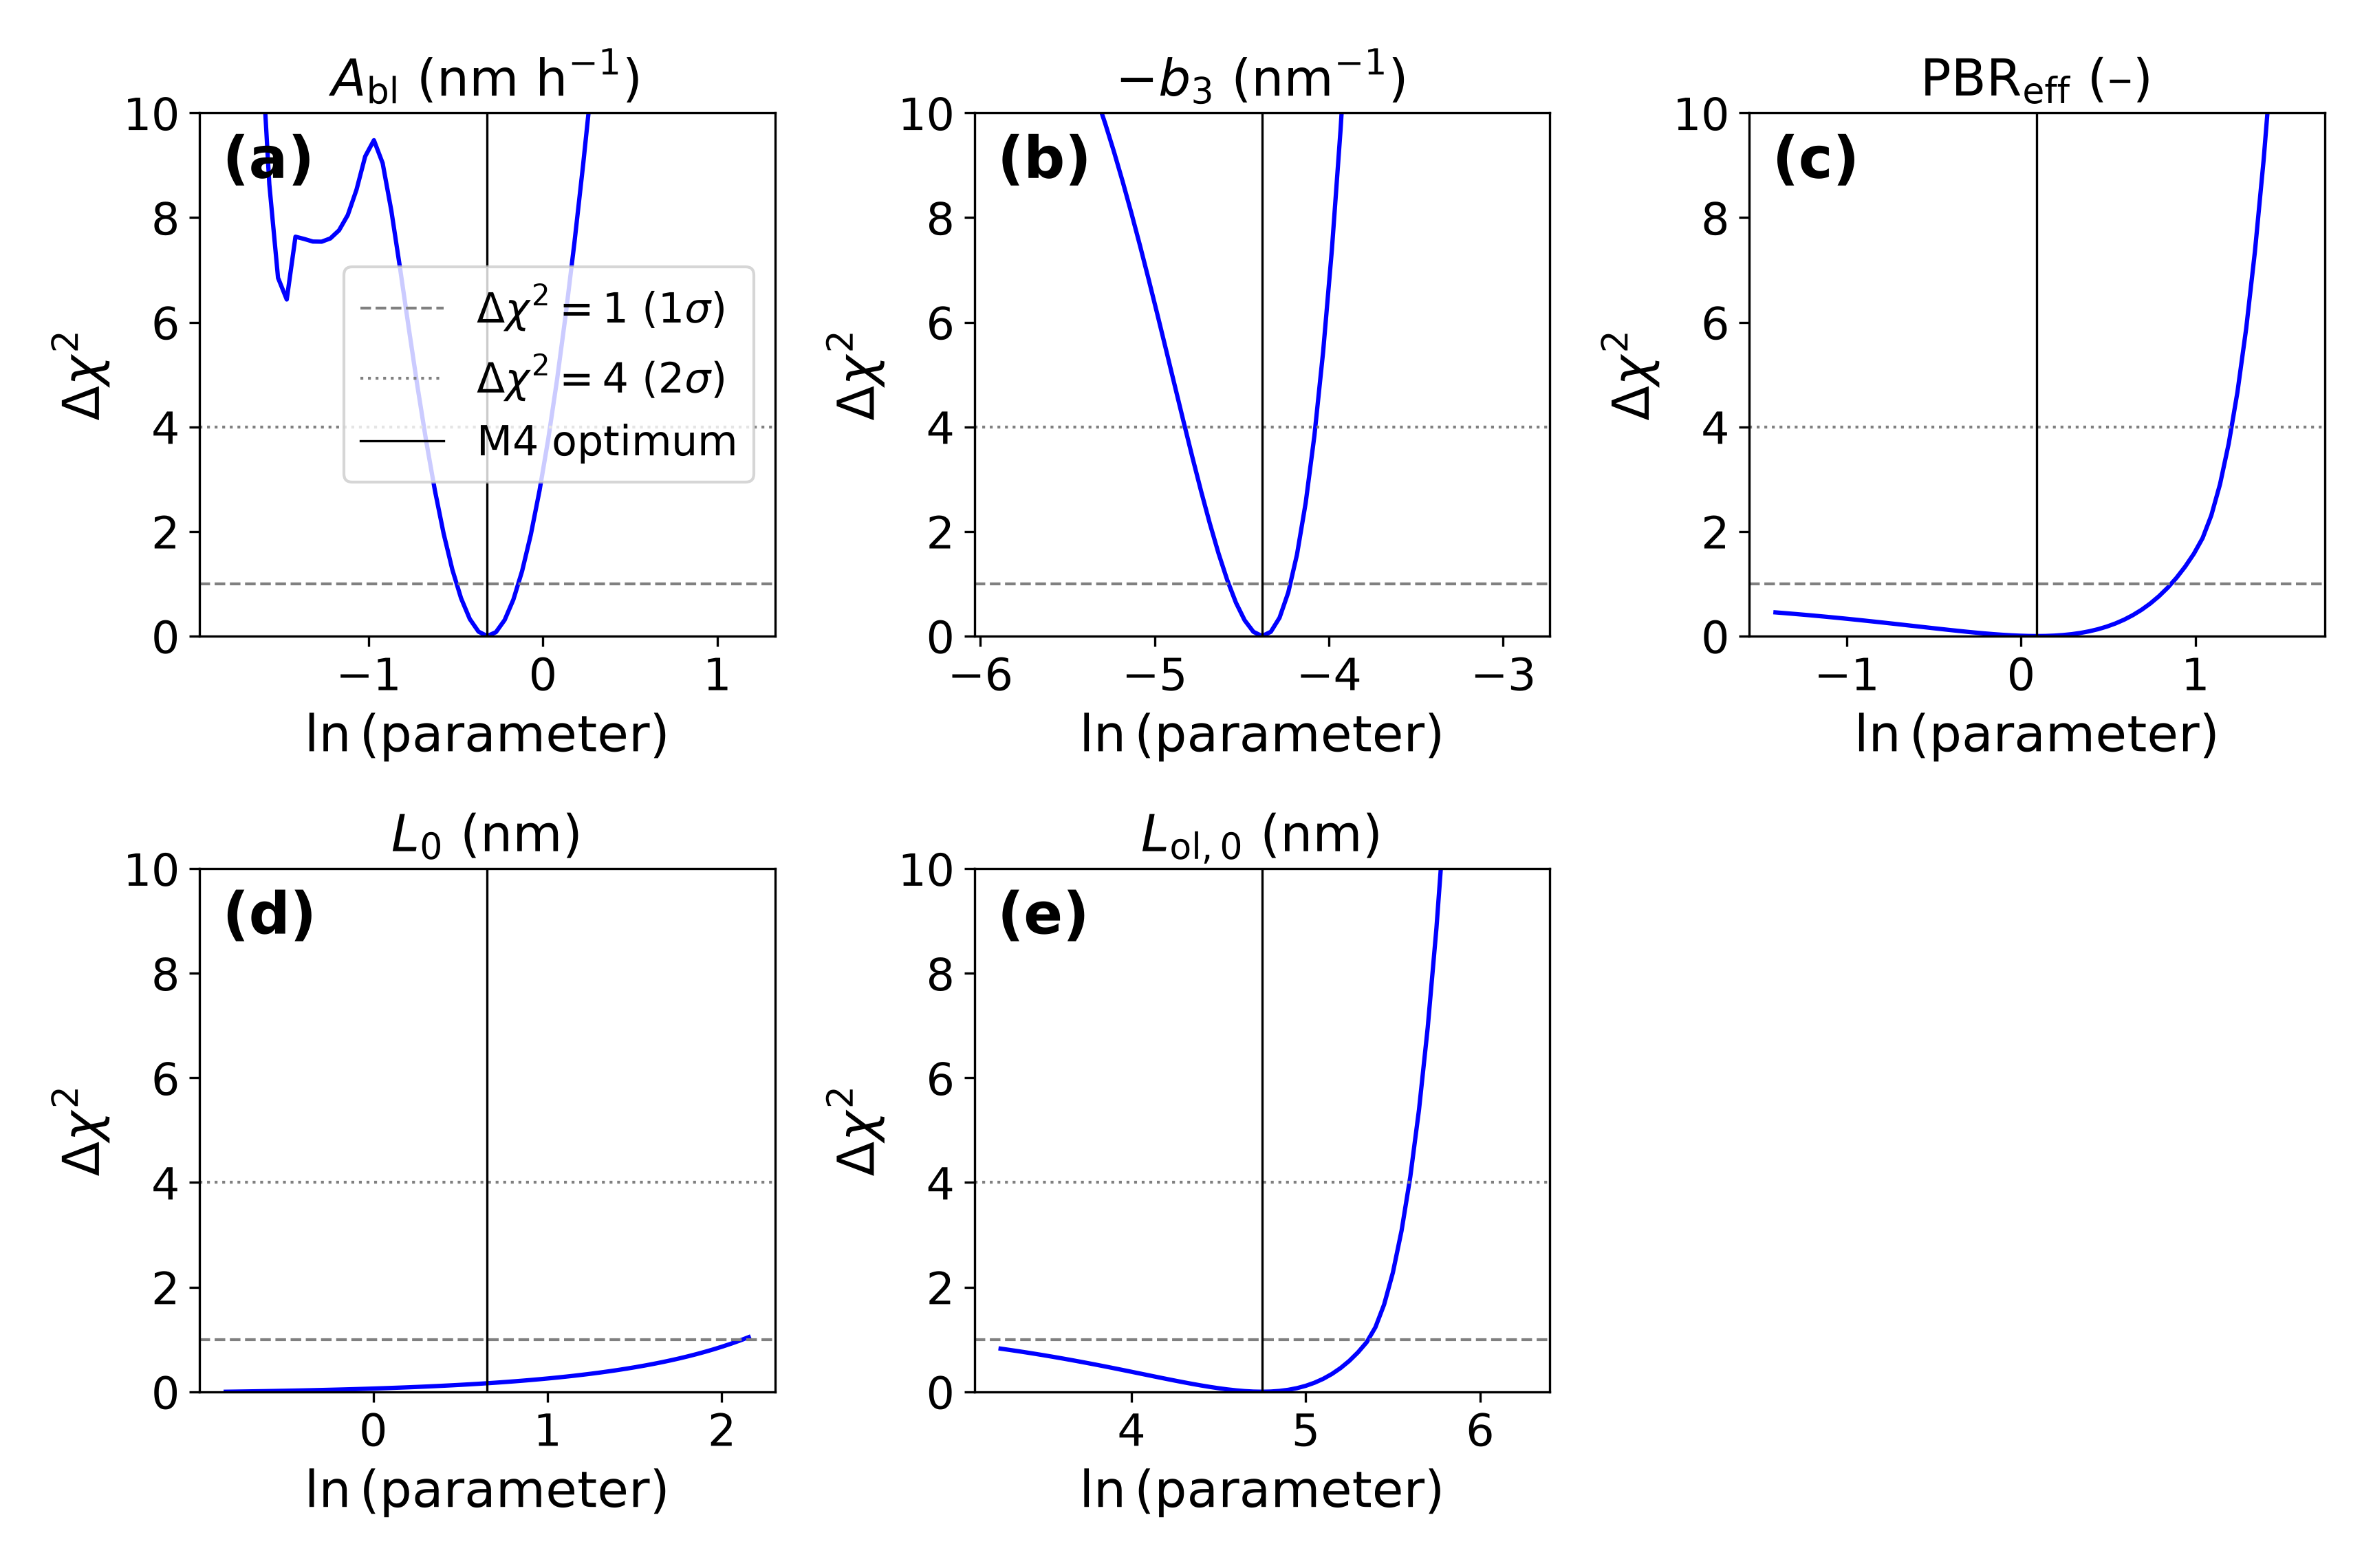
\includegraphics[width=\textwidth]{figures/fig4_profile_likelihood.png}
\caption{Profile-likelihood identifiability map: $\Delta\chi^2$ over
the data residuals versus each M4 parameter (natural-log abscissa),
with the 1$\sigma$ ($\Delta\chi^2 = 1$) and 2$\sigma$
($\Delta\chi^2 = 4$) thresholds marked.}
\label{fig:profile}
\end{figure}

For a parameter carrying a prior, the profile alone cannot separate data
leverage from prior leverage, because both are centred where the prior
is. The direct test is to move the prior and see whether the estimate
follows (Table~\ref{tab:priortest}). $L_0$ follows it completely:
widening its prior fivefold moves the estimate from 1.92 to 1.14~nm
(41\%), and removing it drives $L_0$ to zero, the likelihood having no
interior optimum at all. $\mathrm{PBR}_\text{eff}$ behaves in the
opposite way. It carries no prior here, so the test is run in reverse:
imposing the prior this analysis previously used, centred on 1.05 with
$\sigma_{\ln} = 0.20$, moves the estimate only from 1.096 to 1.051
(4.1\%) and leaves the data $\chi^2$ at 5.79. The likelihood therefore
does define an interior optimum for this parameter, and the former prior
was displacing it by about 4\% rather than creating it. This is the test
that licenses reading $\mathrm{PBR}_\text{eff} \approx 1.10$ as a weak
but genuine data statement while reading $L_0$ as prior-set.

\begin{table}[htbp]
\centering
\caption{Prior-leverage test. Each row refits M4 with the Gaussian
log-space prior widths of Eq.~\eqref{eq:objective} modified as shown
(``off'' = prior removed). A data-determined parameter does not move when
its prior is relaxed; a prior-set one drifts or loses its optimum.}
\label{tab:priortest}
\small
\begin{tabular}{lccccc}
\toprule
Prior setting & $\sigma_{\ln \text{PBR}}$ & $\sigma_{\ln L_0}$ & $\mathrm{PBR}_\text{eff}$ & $L_0$ (nm) & $\chi^2_\text{data}$ \\
\midrule
As fitted (baseline) & --- & 0.60 & 1.096 & 1.924 & 5.79 \\
Impose PBR 1.05, $\sigma=0.20$ & 0.20 & 0.60 & 1.051 & 1.924 & 5.79 \\
Impose PBR 1.05, $\sigma=1.00$ & 1.00 & 0.60 & 1.069 & 1.924 & 5.79 \\
$L_0$ prior $\times5$ & --- & 3.00 & 1.097 & 1.144 & 5.71 \\
$L_0$ prior off & --- & --- & 1.098 & 0.000 & 5.58 \\
Both (impose PBR, $L_0$ off) & 0.20 & --- & 1.051 & 0.000 & 5.59 \\
\bottomrule
\end{tabular}
\end{table}

The 1000-member parametric bootstrap cross-validates these conclusions by
an independent method (Fig.~\ref{fig:ensemble}), and the two weakly
constrained parameters fail it in opposite directions. For the sharply
identifiable growth prefactor and field exponent the bootstrap and
profile intervals agree closely. For $L_0$ the bootstrap spread
($\pm0.036$~nm) is far narrower than the profile interval; this is not a
tighter constraint but an artifact of the bootstrap perturbing only the
data while the profile explores the full parameter range---when the data
have no leverage, every resampled refit collapses onto the same prior.
$\mathrm{PBR}_\text{eff}$, now unconstrained by any prior, shows the
opposite signature: a bootstrap standard deviation of 0.93 on a central
value of 1.10, with the estimate collapsing toward zero in a sizeable
minority of replicates (16th percentile $5\times10^{-9}$). Its profile
interval [0.245, 2.32] and its bootstrap spread agree that three
exposure times pin this parameter only to within about an order of
magnitude. The initial outer-layer thickness sits between these cases:
its profile is sharp ($\Delta\chi^2 = 58$) but its bootstrap is not
($110 \pm 75$~nm, 16th percentile 17~nm), because
$L_\text{ol,0}$ and $\mathrm{PBR}_\text{eff}$ trade off against each
other in the outer-layer data and a resampled replicate can move along
that trade-off at little cost in $\chi^2$. The profile-likelihood
interval, not the bootstrap spread, is the honest uncertainty statement
for $L_0$; for $\mathrm{PBR}_\text{eff}$ the two methods agree that the
constraint is weak; and for $L_\text{ol,0}$ the wider bootstrap should
be preferred, since it is the one that samples the trade-off. All three
verdicts are consequences of the same shortage of exposure times.

\begin{figure}[htbp]
\centering

\includegraphics[width=\textwidth]{figures/fig5_uncertainty_ensemble.png}
\caption{Bootstrap ensemble versus profile likelihood: 1000-member
parametric bootstrap distribution for each M4 parameter, compared
against the profile-likelihood 1$\sigma$ band.}
\label{fig:ensemble}
\end{figure}

\subsection{Validating the neural inversion, and a failure mode specific
to sparse data}\label{sec:pinn}

Because the reduced kinetics have a closed-form solution, this problem
admits something that most physics-informed inverse problems do not: an
exact reference against which the neural inversion can be graded rather
than merely trusted. This section uses that reference twice---once to
establish that the hard-mode inversion is interchangeable with a
classical fitter, and once to expose a soft-mode failure that the
training loss does not reveal.

Applied to the real dataset, the hard-mode neural inversion recovers the
deterministic M4 optimum to within 0.6\% on every parameter, and its
trajectory $\chi^2$ of 5.79 matches the classical baseline exactly
(Table~\ref{tab:f1}). Its recovery behavior was first validated on
synthetic data generated from known ground-truth kinetics with 2\%
relative noise at the same exposure times: recovery deviations are
1.37\% (growth prefactor), 3.39\% (field exponent), 0.59\%
(Pilling--Bedworth ratio), 11.06\% (initial barrier-layer thickness),
and 0.16\% (initial outer-layer thickness). The one large deviation
lands on exactly the parameter the profile-likelihood analysis flags as
unidentifiable---a direct cross-validation of the identifiability
finding by an independent method. A 50-member subset of the bootstrap
re-solved through the hard-mode inversion gives spreads statistically
consistent with the 1000-member deterministic ensemble (growth
prefactor $0.74 \pm 0.12$ deterministic, $0.76 \pm 0.14$
physics-informed), confirming the two fitters are interchangeable.

The soft-mode inversion behaves differently. Trained on the same data,
the joint field-and-parameter optimization settles into an equilibrium
at which the data loss is essentially zero while the governing equation
along the recovered trajectory is not satisfied to the precision the
low data loss suggests. Re-solving the recovered parameters through the
exact forward solution exposes the inconsistency directly: the
trajectory's own $\chi^2$ is 0.21, but the same parameters evaluated
through the exact solution give $\chi^2 = 16.6$
(Table~\ref{tab:f1})---a factor of roughly 80 apart.
Increasing the fixed weight on the physics residual does not resolve
this, because the adaptive loss aggregator renormalizes relative term
weights during training; an independent reweighting toward the data
term reproduces the same signature (trajectory 0.67 versus closed-form
15.6). The specific values vary from training run to run, but the
one-to-two-orders-of-magnitude signature is stable (SI, Section~S4.4). We term
this failure mode F-1 and attribute it to the gradient geometry near
the data manifold: once the data loss is near zero, the physics-residual
gradient is too small to pull the trajectory off that manifold. This
mechanism, and the expectation that dense data would prevent the
imbalance, are offered as a working explanation consistent with the
observations rather than as a demonstrated result.

\begin{table}[htbp]
\centering
\caption{F-1 self-consistency exhibit: trajectory $\chi^2$ versus
closed-form $\chi^2$ at the recovered parameters (seed-0 runs; see SI
Section~S4.4 for run-to-run variability).}
\label{tab:f1}
\small
\begin{tabular}{llccc}
\toprule
Inverse mode & Note & $\chi^2$ traj. & $\chi^2$ closed-form & Self-consistent \\
\midrule
Hard (real data) & physics exact by construction & 5.795 & 5.79 & yes \\
Soft, $\lambda_\text{phys}=10^3$ & joint field+parameter & 0.21 & 16.64 & no \\
Soft, $\lambda_\text{data}=10$ & joint field+parameter & 0.67 & 15.57 & no \\
\bottomrule
\end{tabular}
\end{table}

The practical fix is the hard-mode construction, available for the
zero-dimensional kinetics but not, in general, for the spatial
extension. For soft-mode inversions we therefore apply, and propose for
reporting alongside any physics-informed inverse result, a
self-consistency check: re-solve the recovered parameters through an
independent physics-exact forward solve (closed form, Runge--Kutta, or
Newton iteration) and report the resulting $\chi^2$ next to the
trajectory $\chi^2$. In our experience this is the only test among
those we tried that reliably distinguishes a trustworthy soft-mode fit
from an F-1 failure without requiring a hard-mode alternative to exist;
its acceptance rule is a stated heuristic (SI, Section~S4.4).

Finally, both neural backbones pass the 0.5\% forward acceptance
criterion under identical settings (relative $L^\infty$ errors 0.14\%
and 0.12\% for the two thickness fields with the multilayer-perceptron
backbone, 0.11\% and 0.04\% with the Kolmogorov--Arnold-network
backbone). This is a parity result: on this problem, backbone choice
does not materially change forward accuracy.

\subsection{Spatial extension: defect transport and composition}\label{sec:spatial}

Veile et al.'s line scans resolve full composition-versus-depth
profiles that the zero-dimensional fit never uses. We therefore extend
the model spatially---resolving oxygen- and cation-vacancy transport
across the barrier layer under the already-identified kinetics---and
use the resulting composition predictions as an independent cross-check
against data the fit never saw. The transport problem admits no
differentiable-integrator shortcut of the kind the zero-dimensional
kinetics allow, so the spatial solves use the soft-mode field
representation; it is verified against an independent Newton solve on
the same node set, which for this steady problem is both cheaper and
more accurate, so the comparison below grades the neural solver rather
than relying on it. Every kinetic parameter entering this section is
frozen at its zero-dimensional value.

Before any spatial inversion, a synthetic identifiability gate asks
which spatial quantities the dataset could constrain at all, using an
instrument model with position jitter, compositional noise, and,
critically, the scan-to-scan physical heterogeneity Veile et al.'s
replicate scans exhibit (SI, Section~S2.5; omitting the heterogeneity
term produces a spuriously optimistic verdict for every parameter).
Twenty replicate synthetic experiments (Table~\ref{tab:t2a}) show that
the barrier-layer thickness, interfacial transition widths, nickel-zone
amplitude and width, and in-layer chromium fraction are identifiable
(replicate relative standard deviations 2--19\%), while the in-layer
defect-transport composition gradient---the one quantity the spatial
extension uniquely adds---is weak (47\%, with a minimum statistically
detectable gradient of 0.93 absolute weight percent across the layer).
The spatial model's inverse scope is restricted accordingly, and the
defect-transport gradient is treated as a forward prediction, not a
fitting target.

\begin{table}[htbp]
\centering
\caption{Synthetic identifiability gate for the spatial shape
parameters: 20-replicate recovery under the instrument and
heterogeneity model of SI Section~S2.5. RSD is the replicate relative
standard deviation of the recovered parameter; the verdict thresholds
are 25\% (identifiable) and 50\% (weak). The $L_\text{bl}$ truth value is
the 480-h kinetic-fit output of Table~\ref{tab:leverage} rounded to
134.0~nm.}
\label{tab:t2a}
\small
\begin{tabular}{llcccl}
\toprule
Shape param. & Physics mapping & Truth & Unit & RSD & Verdict \\
\midrule
$L_\text{bl}$ & kinetic-fit output & 134.0 & nm & 2\% & identifiable \\
$w_\text{int}$ & solid-state interdiffusion & 5.0 & nm & 17\% & identifiable \\
$w_\text{out}$ & outer-interface kinetics & 8.0 & nm & 19\% & identifiable \\
$A_\text{Ni}$ & Ni exclusion ratio & 25.0 & wt\% & 7\% & identifiable \\
$w_\text{Ni}$ & Ni exclusion + transport & 35.0 & nm & 8\% & identifiable \\
$f_\text{Cr,bl}$ & interfacial flux ratios & 45.0 & wt\% & 2\% & identifiable \\
$g_\text{bl}$ & defect-transport gradient & 1.0 & wt\% & 47\% & weak \\
\bottomrule
\end{tabular}
\end{table}

The steady-state transport problem, solved by Newton iteration on a
spectral collocation grid and by an NSEM forward solve, agrees with its
analytic reference to $8.9\times10^{-16}$ (oxygen vacancies) and
$2.2\times10^{-13}$ (cation vacancies); the NSEM solve agrees with the
Newton reference to $2.5\times10^{-4}$ and $5.4\times10^{-5}$ relative
error (Fig.~\ref{fig:steady}). The verification also establishes a
structural identifiability result: the steady nondimensional profile
shape depends only on the P\'eclet-type group
$\text{Pe} = |z|\gamma \varepsilon_f L$, fixed by the zero-dimensional
fit, and not on the defect diffusivity. This was confirmed numerically,
not only by inspection of the equations: solving the identical problem
with the diffusivity varied over four orders of magnitude leaves the
profile shape unchanged to machine precision, while the absolute
concentration scale---invisible to a composition measurement such as
EDX---scales inversely with diffusivity exactly as the equations
predict. Quasi-steady composition measurements therefore cannot
constrain the defect diffusivity; only genuinely transient early-time
composition data would carry diffusivity sensitivity, through the
migration transit times quantified below. This structural argument
independently corroborates the statistical gate above.

\begin{figure}[htbp]
\centering

\includegraphics[width=\textwidth]{figures/fig8_steady_spatial.png}
\caption{Steady spatial solve. (a)~Steady-state nondimensional profile
shape with diffusivity scaled by $0.01\times$ to $100\times$; the
curves coincide to machine precision, confirming the
diffusivity-cancellation result. (b)~Verification ladder: Newton versus
analytic, and NSEM versus Newton, for both defect species; horizontal
lines mark the $10^{-10}$ and 0.5\% acceptance bounds.}
\label{fig:steady}
\end{figure}

The transient extension, solved on a moving Landau-transformed domain
tracking the growing layer, quantifies an approximation every
zero-dimensional PDM application makes implicitly: that the defect
profile equilibrates instantaneously to its steady shape. At the end of
the 480-h window the fast oxygen-vacancy species (migration transit
time of order 5~h) lags its quasi-steady shape by 0.69\%, and the
slower cation-vacancy species (transit time of order 36~h) by 5.79\%
(SI, Fig.~S2)---both inside the acceptance tolerances used here, and
both scaling with the ratio of transit time to growth timescale as the
physics predicts. We are not aware of a prior explicit quantification
of this quasi-steady error in the PDM literature.

The composition-map prediction uses no free parameters, and its two
components test different things. The predicted chromium plateau inside
the barrier layer, 46.7 weight percent against a measured plateau of
approximately 45 weight percent, follows from spinel stoichiometry
alone---the FeCr$_2$O$_4$ assignment~\citep{ziemniak2003spinel} Veile
et al.\ report as one of several candidate chromium-rich spinels
(alongside Cr$_2$O$_3$, Fe$_2$CrO$_4$, and NiCr$_2$O$_4$) consistent
with their X-ray photoelectron spectroscopy results---and therefore
validates a plausible phase assignment, not the kinetics. The kinetic
content is in the layer widths, which the frozen kinetics match to
within $+22\%$, $-20\%$, and $+3\%$ at the three exposure
times (Fig.~\ref{fig:composition})---agreement at the tens-of-percent
level from a zero-free-parameter prediction, not a quantitative
reproduction---extracted from prediction and
measurement by the same criterion Veile et al.\ use (chromium trace
exceeding its far-field baseline by three weight percent). The
predicted in-layer defect gradient---1.45, 0.96, and 0.46 absolute
weight percent at 72, 168, and 480~h---straddles the 0.93 weight
percent detection floor from the identifiability gate: marginally
detectable at the earliest exposure, undetectable by the latest.

\begin{figure}[htbp]
\centering

\includegraphics[width=\textwidth]{figures/fig10_composition_edx.png}
\caption{Zero-free-parameter composition-map prediction against Veile
et al.'s measured EDX features at (a)~72, (b)~168, and (c)~480~h.
Curves are predicted composition profiles (O, Cr, Fe, Ni; weight
percent) versus depth from the metal/barrier-layer interface; overlays
mark the measured features compared: Cr-layer width (shaded band), Cr
plateau level ($\sim$45~wt\%, dotted), and the 72-h Ni-peak amplitude
($23.7\pm7.0$~wt\%, error bar). Full digitized EDX traces are not
available, so the comparison is feature-based.}
\label{fig:composition}
\end{figure}

\subsection{The nickel enrichment zone}\label{sec:nickel}

The nickel zone is the one feature of the duplex scale that the
identified kinetics do not describe, and the reason is instructive. An
exact moving-frame nickel-transport model with a constant effective
mobility (SI, Section~S3), fitted to the measured zone widths and the
72-h peak amplitude, is \emph{rejected} by the data: $\chi^2 = 25.7$ on
one degree of freedom. The rejection is one of shape, not scale---the
model predicts a zone width growing monotonically with exposure, while
the measured widths are approximately flat (31, 43, 36~nm at 72, 168 and
480~h). Because parameter values and nested-model $\Delta\chi^2$
comparisons obtained under a structurally rejected model are not
interpretable as estimates or as evidence, the fitted values and the
nested-model comparison are reported in the SI (Section~S3.1,
Table~S6) and are not carried into the Discussion as findings.

Two statements about the nickel zone do survive independently of that
fit, and they are the section's result. First, the measured widths are
flat within scatter across a factor of 6.7 in exposure time, which no
constant-mobility transport model of this class can produce: any such
model predicts a width growing as the square root of time or faster.
Second, any effective mobility consistent with the observed zone
scale---a zone tens of nanometres wide developing over hundreds of
hours---is of order $10^{-17}$~cm$^2$/s, which exceeds extrapolated
lattice self-diffusion of nickel in austenite at 513~K by many orders of
magnitude. This is a scale argument, independent of the fitted value: the
zone-forming transport must be short-circuit or defect-flux mediated
rather than lattice-diffusive. Taken together, the two point to a
time-decaying or interface-coupled mobility.

That mechanism is exactly what three exposure times cannot resolve. Two
physically motivated one-parameter extensions were tested---a
defect-flux-coupled effective mobility tied to the identified growth
kinetics, and a finite-capacity interfacial trapping closure---and both
fail a twenty-replicate synthetic identifiability gate before touching
real data (SI, Table~S7): the flux-coupled closure's new parameter is
recoverable but destabilizes the already-identified transport parameters
past threshold, and the finite-capacity closure's parameter is not
recoverable at all (SI, Section~S3.2). A forward-only scan across the
flux-coupled closure's plausible range confirms no single value is
simultaneously shape-correct
and a quantitative improvement. Resolving the nickel zone is therefore
left as a target for denser exposure-time data, and is one more instance
of the exposure-time limitation that recurs throughout this paper.

\subsection{Long-time extrapolation and operating-envelope sensitivity}\label{sec:predictions}

At ten years---a factor of roughly 180 beyond the 480-h calibration
window---the identified model predicts a barrier-layer thickness of
535~nm, with bootstrap 68\% and 95\% intervals of [482, 606] and [447,
704]~nm (Fig.~\ref{fig:longtime}). These bands quantify parametric
uncertainty conditional on the M4 model structure and on the reported
standard errors; under the maximal error-scale correction of
Section~\ref{sec:ladder} ($s = 2.4$, applied in log space) the 95\%
interval widens to approximately [340, 1040]~nm. Extrapolating Veile
et al.'s published power-law coefficients over the same horizon instead
predicts 1853~nm (a factor of 3.5), and the weighted-refit power law
3375~nm (a factor of 6.3; bootstrap 68\% interval on the ratio [5.6,
7.0]). Either power-law prediction lies outside the mechanistic band
even after the maximal inflation. The divergence is the practical
consequence of the constant-volume-coupled growth law saturating
logarithmically while the power law, fit independently to each layer,
extrapolates indefinitely.

\begin{figure}[htbp]
\centering
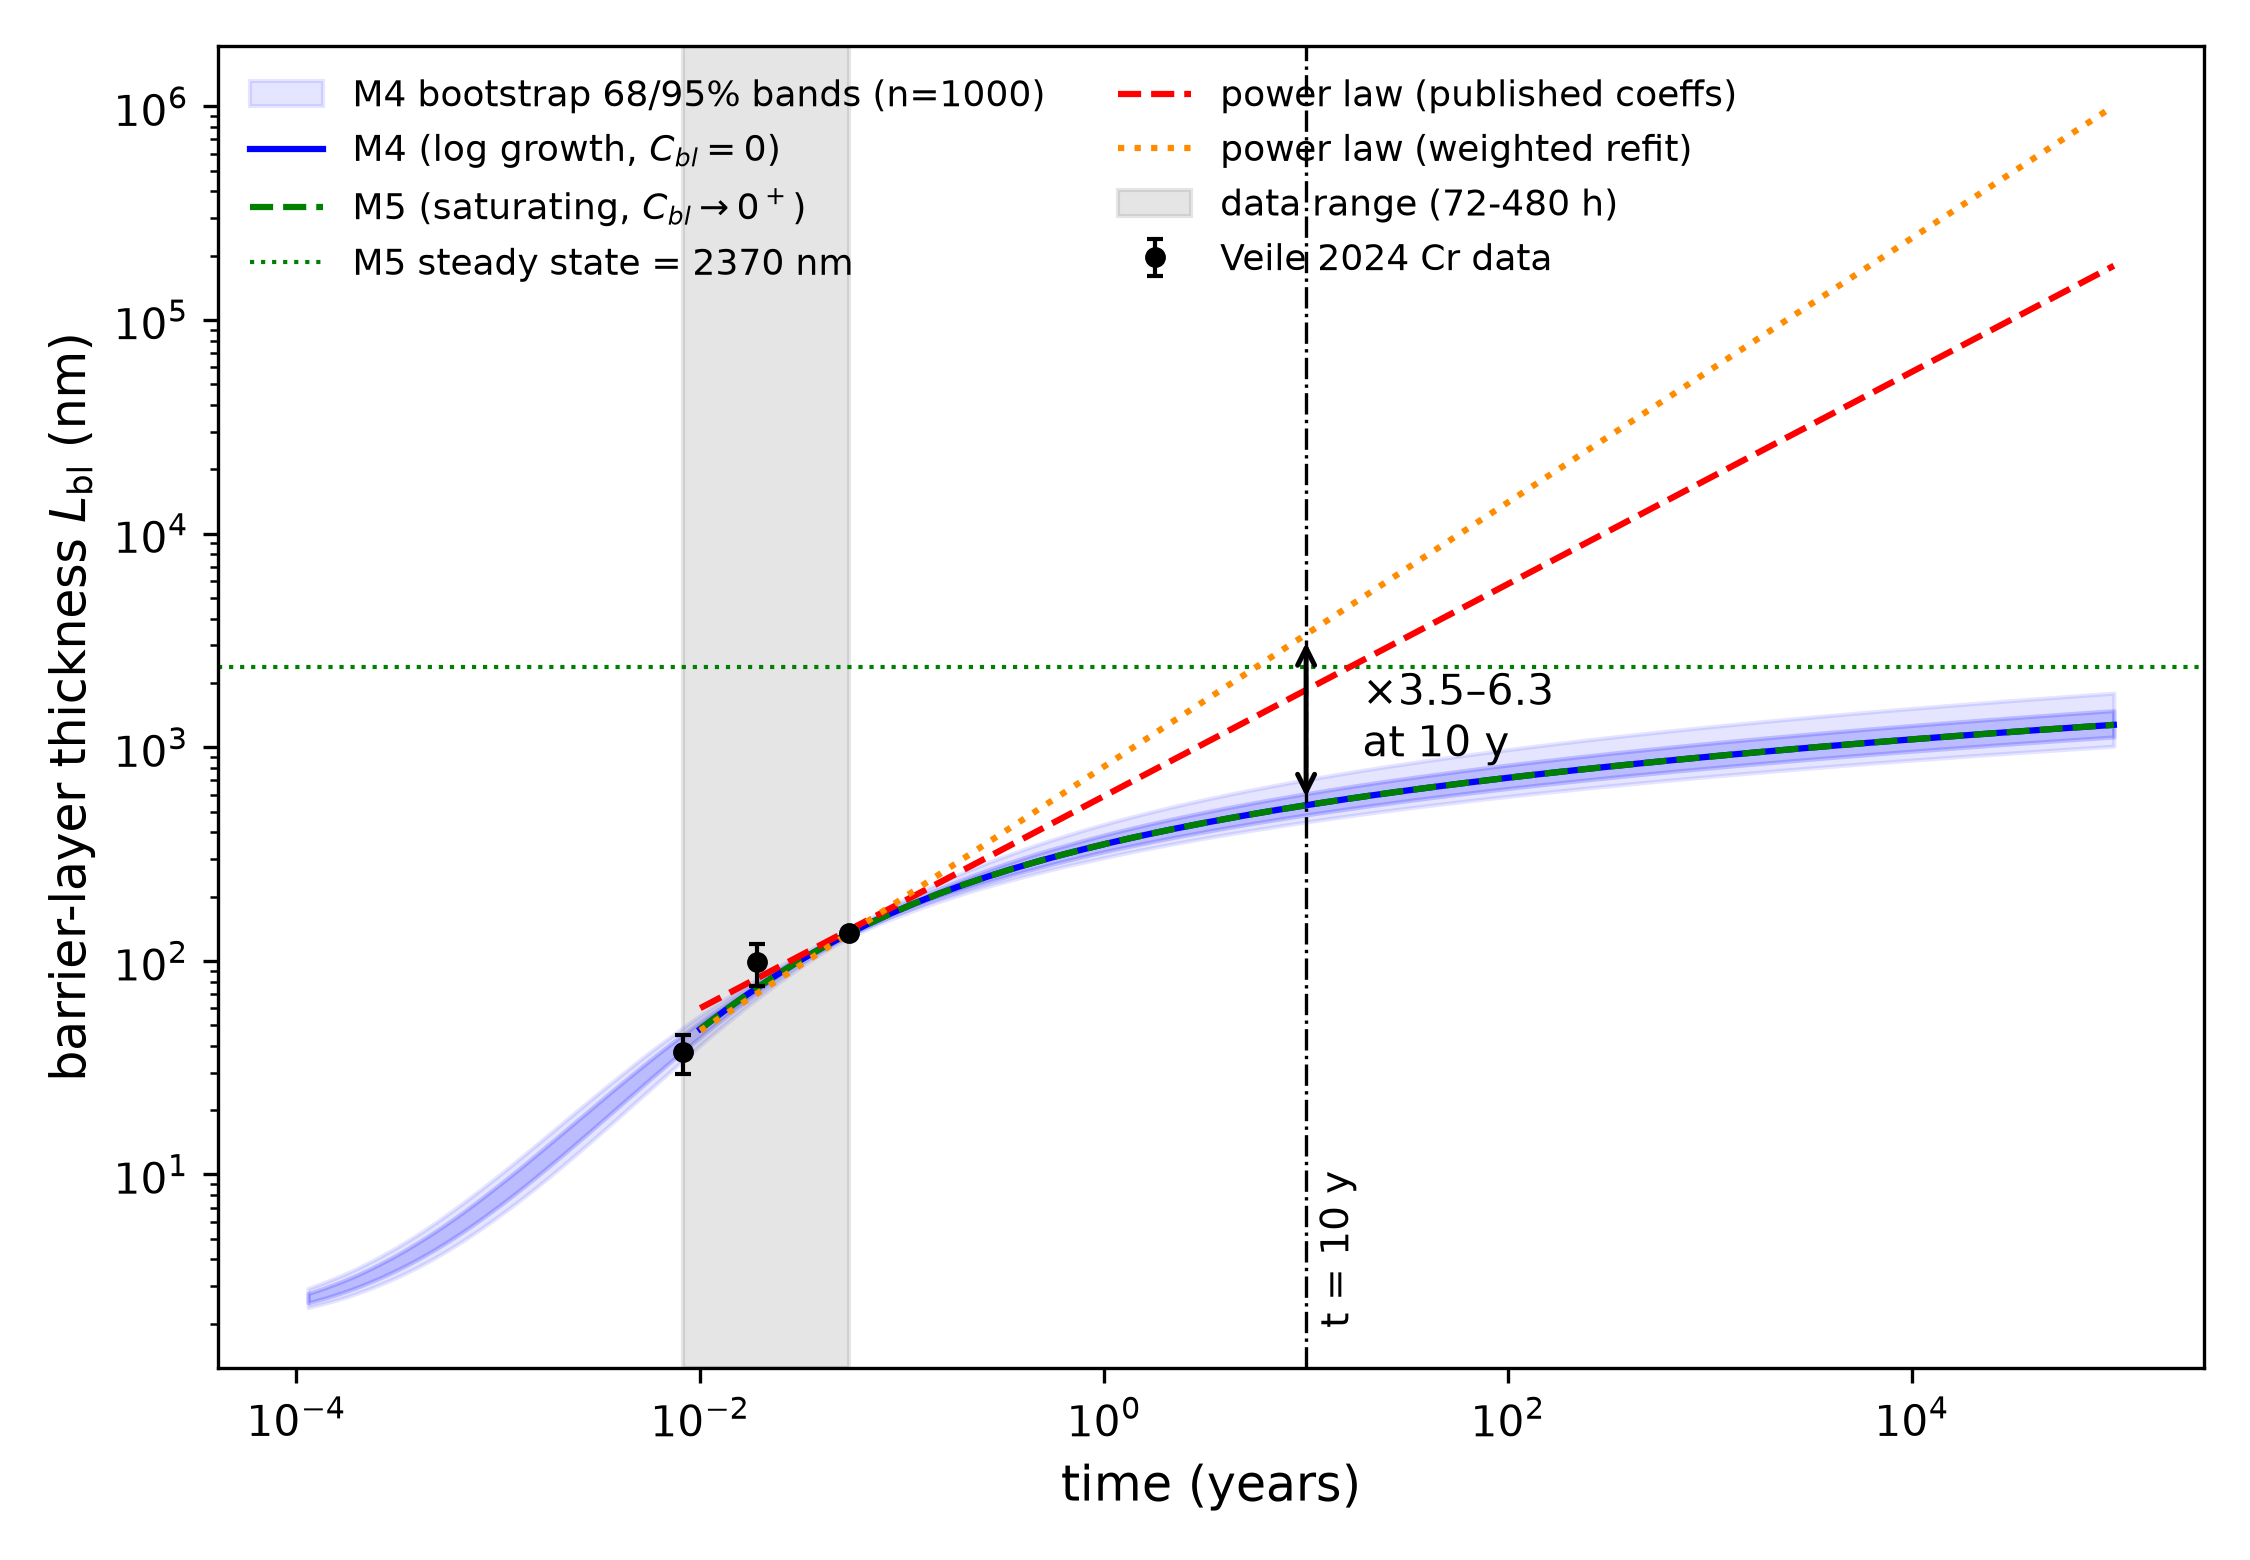
\includegraphics[width=\textwidth]{figures/fig6_long_time.png}
\caption{Long-time prediction with propagated parametric uncertainty:
M4 (logarithmic growth) versus M5 (saturating branch) versus the two
power-law variants, to $10^5$~years. Shaded bands are the 68\% and 95\%
intervals of the 1000-member parametric bootstrap propagated through
the M4 closed form, conditional on the M4 model structure and the
reported standard errors; the M5 curve is indistinguishable from M4 at
all feasible exposures. The vertical line marks the ten-year horizon.}
\label{fig:longtime}
\end{figure}

The model's own two long-time branches---unbounded logarithmic growth
(M4) versus eventual saturation (M5)---track within about five percent
of each other out to $10^5$~years: no feasible exposure experiment
could distinguish them from thickness data, the prediction-space
restatement of the dissolution-rate unidentifiability of
Section~\ref{sec:identifiability}. Discriminating mechanistic from
power-law extrapolation is, by contrast, feasible. Under a conservative
scatter model for a future campaign (the worst observed chromium
scan-level relative standard deviation, 22\%, averaged over three
scans, giving a 12.7\% standard error), the separation between the two
predictions first exceeds twice that scatter at 2551~h with the
published coefficients (1437~h refit) and three times at 4011~h
(2024~h refit). These thresholds compare the separation to future
measurement scatter alone, and so understate the required exposure. Adding
the mechanistic prediction's own parametric uncertainty (the
1000-member bootstrap propagated to each exposure time) and the
power-law fit uncertainty (an equivalent bootstrap of the weighted refit)
in quadrature moves the 2$\sigma$ threshold to 2996~h with the published
coefficients and 1944~h with the refit, and the 3$\sigma$ threshold to
5133~h and 5850~h respectively. A designed exposure of roughly 3000~h is
therefore the realistic requirement for 2$\sigma$ discrimination against
the full error budget, and roughly 5000--6000~h for 3$\sigma$; the
scatter-only numbers should be read as the optimistic bound they are.

Because the dataset was collected at a single temperature and oxygen
level, the model's sensitivity is mapped across a scanned operating
envelope of 200--285$^\circ$C at 7~MPa and 0.01--8~ppm dissolved
oxygen---deliberately extended beyond normal-water-chemistry oxygen
levels ($\sim$0.2--0.4~ppm) to bound off-normal chemistry. The upper
temperature bound is the liquid-phase stability limit at 7~MPa
($T_\text{sat} \approx 286^\circ$C), so nominal BWR coolant temperature
($\approx 288^\circ$C at operating pressure) sits essentially at the
edge of the scanned box, not comfortably inside it. The temperature
channel follows the rate-constant structure of the supercritical-water
formulation~\citep{li2020scwpdm}: the rate-determining constant scales
as $\exp[-\alpha_3 \Delta G^0_R/R\,(1/T - 1/T_0)]$, so the effective
Arrhenius activation energy is $\alpha_3 \Delta G^0_R$, and with the
standard Gibbs energy of the growth reaction unmeasurable from
single-temperature data, $\Delta G^0_R$ must be scanned explicitly. The
scan is set by the effective activation energy it implies rather than by
$\Delta G^0_R$ itself: at $\alpha_3 = 0.12$ the range
25--417~kJ/mol corresponds to $\alpha_3 \Delta G^0_R = 3$--50~kJ/mol,
which spans both the low values implied by transferring a
supercritical-water transfer coefficient and the several tens of kJ/mol
reported for weight-gain kinetics of austenitic steels in
high-temperature water. Scanning only the lower part of that range would
build the robustness conclusion on the assumption most favourable to it.
A field-attenuation channel is tied to the same
temperature dependence, and the dissolved-oxygen channel is an
ideal-Nernst shift of the growth prefactor---an explicit lower bound on
the true corrosion-potential response (Section~\ref{sec:discussion}).

Across this envelope (Fig.~\ref{fig:sensitivity},
Table~\ref{tab:envelope}), the predicted barrier-layer thickness varies
by a factor of 1.20 to 2.92 at 480~h and 1.19 to 1.56 at ten years,
depending on the scanned effective activation energy; temperature
dominates through the combined Arrhenius and field-attenuation channels,
while dissolved oxygen contributes a mild tilt. Two features of this
result matter more than the headline range. First, the sensitivity is
strongly conditional on the activation energy: over the low
3--12~kJ/mol sub-range the ten-year envelope factor is a nearly
negligible 1.19--1.25, but at 50~kJ/mol it is 1.56, and the 480-h factor
roughly doubles from 1.42 to 2.92. Second, the ten-year factor is
consistently smaller than the 480-h factor, because logarithmic growth
compresses prefactor differences at long times---the robustness of the
\emph{long-time} prediction is a property of the growth law, and is not
inherited from a robustness of the short-time behaviour. The long-time
prediction is therefore moderately, not strongly, sensitive to operating
condition across the full plausible activation-energy range, and a factor
of about 1.6 should be carried alongside the parametric band of
Fig.~\ref{fig:longtime} rather than the 1.25 the narrow scan alone would
suggest.

\begin{table}[htbp]
\centering
\caption{Operating-envelope spread of the predicted barrier-layer
thickness over the scanned box (200--285$^\circ$C at 7~MPa, 0.01--8~ppm
O$_2$), as a function of the assumed effective Arrhenius activation
energy $\alpha_3\Delta G^0_R$. The first three rows are the
originally scanned range; the last two extend it to the values reported
for weight-gain kinetics on austenitic steels in high-temperature water.}
\label{tab:envelope}
\small
\begin{tabular}{cccccc}
\toprule
$\Delta G^0_R$ & $\alpha_3\Delta G^0_R$ & \multicolumn{2}{c}{$L_\text{bl}$(480~h)} & \multicolumn{2}{c}{$L_\text{bl}$(10~y)} \\
\cmidrule(lr){3-4}\cmidrule(lr){5-6}
(kJ/mol) & (kJ/mol) & range (nm) & factor & range (nm) & factor \\
\midrule
25 & 3 & 123--147 & 1.20 & 492--583 & 1.19 \\
50 & 6 & 119--151 & 1.27 & 487--588 & 1.21 \\
100 & 12 & 113--159 & 1.42 & 479--598 & 1.25 \\
250 & 30 & 93--185 & 1.99 & 452--627 & 1.39 \\
417 & 50 & 73--214 & 2.92 & 423--660 & 1.56 \\
\bottomrule
\end{tabular}
\end{table}

\begin{figure}[htbp]
\centering

\includegraphics[width=\textwidth]{figures/fig7_sensitivity_maps.png}
\caption{Operating-envelope sensitivity maps: predicted $L_\text{bl}$
at (a--d)~480~h and (e--h)~ten years over the scanned envelope
(200--285$^\circ$C, 0.01--8~ppm O$_2$), for $\Delta G^0_R = 25$, 100,
250 and 417~kJ/mol---effective activation energies
$\alpha_3\Delta G^0_R$ of 3, 12, 30 and 50~kJ/mol, spanning the full
plausible range rather than only the low values a transferred
supercritical-water transfer coefficient implies. The marker locates the
Veile et al.\ calibration condition. Each row shares a common color
scale, so the widening spread from left to right is the sensitivity
increasing with activation energy.}
\label{fig:sensitivity}
\end{figure}


\section{Discussion}\label{sec:discussion}

\subsection{Mechanistic reading of the empirical exponents}

The mechanistic model supports a physical reading of Veile et al.'s
fitted exponents that the power-law description cannot offer. The
near-parabolic chromium exponent ($n \approx 0.50$) is the signature of
a barrier layer growing under near-zero dissolution in ultrapure water;
the sub-parabolic iron exponent ($n \approx 0.22$) reflects deposition
constrained by constant-volume coupling to the barrier layer from a
substantial initial precipitate population, rather than independent
iron-layer kinetics. This reading is available regardless of fit
quality, and it is the coupling behind it---not $\chi^2$---that
separates the two descriptions' ten-year predictions by a factor of 3.5
to 6.3.

\subsection{The Pilling--Bedworth ratio and a chromium mass balance}

The identified $\mathrm{PBR}_\text{eff} = 1.096$ is one of the two
quantities the exposure-time data constrain only weakly, and it is worth
being explicit about what it does and does not agree with. An earlier
version of this analysis placed a prior on it centred on 1.05 and
described that centre as the stoichiometric spinel/magnetite value. It is
not. The constant-volume closure that yields 1.05 requires the barrier
layer to draw approximately 30~at\% chromium from an alloy containing
18.8~at\%, which the alloy cannot supply. A chromium mass balance on
X6CrNiNb18-10 with an FeCr$_2$O$_4$ barrier gives
$\mathrm{PBR}_\text{eff} = 2.09$ if every iron atom not retained in the
nickel-enriched zone reports to the outer layer. That figure is the
natural point of comparison, but---as the rest of this section
shows---it is neither unique nor a bound.

The likelihood puts the parameter at 1.10, a factor of 1.9 below that
figure. That gap is not a conflict, for two independent reasons, and
neither of them requires the fit to be wrong.

The first is that 2.09 is not a bound but one value of a
phase-dependent quantity. It follows from assigning the barrier the
composition FeCr$_2$O$_4$, and the photoelectron spectroscopy admits
three further chromium-rich spinels. Carrying the same mass balance
through each of them---using lattice-parameter molar volumes, the
nominal alloy composition, and, in one variant, the nickel routing
fraction identified in Section~\ref{sec:spatial} rather than an
assumption of complete nickel rejection---gives production ratios of
2.05 (FeCr$_2$O$_4$), 2.50 (NiCr$_2$O$_4$), 3.64 (Cr$_2$O$_3$) and 0.52
(Fe$_2$CrO$_4$). The stoichiometrically admissible range is therefore
$[0.52, 3.79]$, and the identified 1.10 lies inside it. Only the
FeCr$_2$O$_4$ assignment produces a discrepancy at all.

The second reason is that, at any fixed phase assignment, the two
numbers are not the same quantity. A mass balance fixes the rate at
which barrier growth \emph{produces} outer-layer oxide. The accepted
model pins $C_x = 0$, so its $\mathrm{PBR}_\text{eff}$ measures net
\emph{accumulation} instead, and the two differ by whatever oxide leaves
for the coolant. Freeing $C_x$ separates them, and doing so shows the
data cannot: imposing the FeCr$_2$O$_4$ value of 2.05 changes $\chi^2$
from 5.79 to 5.67, a \emph{decrease} of 0.12
(Table~\ref{tab:pbrclosure}), paid for by an outer-layer loss rate of
0.24~nm/h and a smaller initial precipitate population, 94 against
116~nm. Profiling $\mathrm{PBR}_\text{eff}$ from 0.5 to 8 in this family
moves $\chi^2$ by 0.89 in total, so the $\Delta\chi^2 = 1$ interval is
the entire scanned range. The reason is structural rather than
statistical: with $L_\text{bl}(t)$ fixed, the outer-layer solution
$L_\text{ol}(t) = L_\text{ol,0} + \mathrm{PBR}_\text{eff}\,
(L_\text{bl} - L_0) + C_x t$ carries three parameters against exactly
three outer-layer observations, so it is saturated and no combination is
preferred.

The correct statement is therefore not that the identification
disagrees with stoichiometry, but that three exposure times cannot
separate oxide production from oxide loss. This also explains an
observation that would otherwise look like a loose end: the M1 and M2
variants, which lack the initial precipitate population, reach
$\mathrm{PBR}_\text{eff} = 2.43$---they are simply at a different point
on the same flat direction. The resolution makes one falsifiable
prediction. If the barrier is FeCr$_2$O$_4$ and stoichiometry holds,
the outer layer must lose about 9~\textmu g of iron per square decimetre
per hour, a magnitude consistent with the corrosion-product release
reported for stainless steels in high-temperature
water~\citep{lister1987release}. Nothing measured here demonstrates it:
this dataset contains no coolant chemistry, and the outer layer's
scan-to-scan scatter is so large that it carries only 5\% of the fit
statistic (Table~\ref{tab:leverage}). A coolant mass balance, or
outer-layer thicknesses at more exposure times, would decide it.

\begin{table}[htbp]
\centering
\caption{Imposing a stoichiometric $\mathrm{PBR}_\text{eff}$ once the
outer-layer loss term $C_x$ is free. The accepted model's value is
recovered at $C_x \approx 0$; every larger value is reached at no cost in
$\chi^2$, paid for by outer-layer loss and a smaller initial precipitate
population. $\chi^2 = 5.79$ for the accepted model.}
\label{tab:pbrclosure}
\small
\begin{tabular}{lcccc}
\toprule
$\mathrm{PBR}_\text{eff}$ imposed & $\chi^2$ & $\Delta\chi^2$ &
$C_x$ (nm/h) & $L_\text{ol,0}$ (nm) \\
\midrule
1.10 \; (accepted model)          & 5.784 & $-0.007$ & $-0.025$ & 120.2 \\
2.05 \; (FeCr$_2$O$_4$)           & 5.671 & $-0.120$ & $-0.241$ & 93.6 \\
2.16 \; (FeCr$_2$O$_4$, Ni routed) & 5.661 & $-0.131$ & $-0.264$ & 90.7 \\
2.43 \; (M1/M2 optimum)           & 5.635 & $-0.157$ & $-0.327$ & 83.0 \\
\bottomrule
\end{tabular}
\end{table}

\subsection{What is, and is not, specific to the stabilized alloy}

The reaction network fitted here contains nothing niobium-specific, and
none of the five identified parameters can be attributed to Nb
stabilization on the evidence presented. It is worth being explicit about
what that means, since the alloy's stabilization is the reason it is used
in reactor internals. The identification is specific to AISI~347 in the
sense that the numbers come from measurements on AISI~347, not in the
sense that the model structure encodes Nb; every parameter is an apparent
quantity for an 18Cr--10Ni austenitic matrix under this environment, and
the same structure fitted to 304 or 316 data in the same environment
would differ only through the fitted values. Distinguishing a genuine
stabilization effect would require the comparison this dataset does not
contain: matched exposures of stabilized and unstabilized grades, in
which NbC precipitates could be shown to alter local chromium
availability at the metal/barrier-layer interface, to nucleate or pin the
inner spinel, or to change the initial film that $L_0$ and
$L_\text{ol,0}$ parametrize. Two of the identified quantities are the
natural place such an effect would appear---the growth prefactor
$A_\text{bl}$, through chromium supply to the growth reaction, and the
initial-condition parameters, through surface and precipitate
structure---and both are reported here with intervals wide enough that a
moderate stabilization effect would be invisible. The claim we make is
therefore that this is the first mechanistic identification for this
alloy in this environment, not that the mechanism identified is peculiar
to the stabilized grade.

\subsection{Field strength and comparison with other systems}

Converting the identified field exponent with
$b_3 = -\alpha_3\chi\gamma\varepsilon_f$ requires the growth-reaction
transfer coefficient, which single-temperature thickness data cannot
supply. At the reference value $\alpha_3 = 0.12$ fit by Li et
al.~\citep{li2020scwpdm} for a ferritic steel in supercritical water,
$\varepsilon_f = 1.7\times10^4$~V/cm; over the physically defensible
range $\alpha_3 \in [0.1, 0.5]$ the derived field spans
$4.1\times10^3$ to $2.1\times10^4$~V/cm. The implied potential drop
across the 480-h barrier layer, $\varepsilon_f L$, is correspondingly
0.06--0.28~V; mixed-potential estimates of the corrosion potential in
oxygenated 288$^\circ$C BWR water are of order 0 to
$+150$~mV on the standard hydrogen electrode (SHE)
scale at 0.2--0.4~ppm
O$_2$~\citep{macdonald1992hwc,lin1996ecp}, which favors the lower end
of the derived range and is one more reason to treat $\varepsilon_f$
here as an order-of-magnitude quantity. Within that reading, the value
sits plausibly between the $\sim10^2$~V/cm of supercritical-water PDM
fits at 500$^\circ$C~\citep{li2020scwpdm} and the $\sim10^6$~V/cm of
room-temperature passive films~\citep{cabrera1949oxidation}; we offer
this ordering as a weak plausibility remark only, since the three
anchors span different alloy classes and film chemistries, and the
nearest-temperature precedents (PDM and mixed-conduction analyses of
304/316 in 280--320$^\circ$C
water~\citep{ss316l_pwr_pdm,bojinov_mcm,ss316ln_pdm2024}) do not report
directly comparable apparent field strengths.

Table~\ref{tab:context} places the identified kinetics in the context
of the high-temperature-water oxide corpus. The inner-layer thickness
trajectory recovered here (41~nm at 72~h to 135~nm at 480~h) is of the
same order as inner-layer thicknesses reported for 304/316 stainless
steels in oxygenated 288$^\circ$C water at comparable
times~\citep{kuang2010oxidation,kim1999oxide}, and the duplex
morphology, inner-layer spinel chemistry, and near-parabolic inner
growth match the established picture for austenitic steels in this
environment~\citep{robertson1991mechanism,stellwag1998mechanism,ziemniak2002corrosion}.
The ten-year prediction of 535~nm has no direct validation data for
AISI~347; we are not aware of published long-term harvested-component
oxide thicknesses for this alloy in BWR conditions, and the prediction
should be read as a testable statement, not a validated one.

\begin{table}[htbp]
\centering
\caption{The identified kinetics in the context of related systems.
Literature thickness entries are indicative orders of magnitude for the
Cr-rich inner layer; field strengths are apparent values as reported by
the cited analyses.}
\label{tab:context}
\footnotesize
\setlength{\tabcolsep}{4pt}
\small
\begin{tabular}{lllll}
\toprule
System & Environment & $T$ ($^\circ$C) & Inner layer & $\varepsilon_f$ (V/cm) \\
\midrule
AISI 347 (this work) & simulated BWR HTW & 240 & 41--135~nm (72--480 h) & $4\times10^3$--$2\times10^4$ \\
304/316 SS & oxygenated HTW~\citep{kuang2010oxidation,kim1999oxide} & 288 & tens--hundreds nm & not reported \\
HCM12A, 316L & supercritical water~\citep{li2020scwpdm} & 500 & $\mu$m scale & $\sim10^2$ \\
Passive metals & ambient aqueous~\citep{cabrera1949oxidation} & 25 & 1--5~nm & $\sim10^6$ \\
\bottomrule
\end{tabular}
\end{table}

\subsection{The nickel zone: an anomalous mobility}

The one nickel result that does not depend on a fitted model is a scale
argument, and it is the mechanistically interesting one. An effective
mobility of order $10^{-17}$~cm$^2$/s---the scale required for a
zone tens of nanometres wide to develop over hundreds of hours at
240$^\circ$C---exceeds extrapolated lattice self-diffusion of nickel in
austenite at 513~K by many orders of magnitude. Whatever transports
nickel at the receding metal/barrier-layer interface is therefore
short-circuit or defect-flux mediated rather than lattice-diffusive.
That is also the class of mechanism whose mobility would decay as the
interface structure coarsens, which is the natural explanation for the
flat measured zone widths that defeat the constant-mobility model
(Section~\ref{sec:nickel}). We stop there: distinguishing candidate
short-circuit mechanisms requires exposure-time resolution this dataset
does not have, and the constant-mobility fit is rejected by the data in
shape, so neither its incorporation ratio nor its nested-model
comparison against a re-precipitation-only outer-layer supply picture
can be offered as evidence either way.

\subsection{Limitations}

The kinetic identification rests on a single temperature and a single
dissolved-oxygen level; the operating-envelope maps are forward
projections under sourced assumptions, not validation against
multi-condition data, which does not exist for this alloy. Three
specific gaps between the calibration environment and an operating
reactor deserve explicit statement beyond the envelope scan. First, the
exposures are unirradiated and static: radiolysis products, especially
H$_2$O$_2$, are known to alter oxide structure and thickness on
stainless steels relative to O$_2$ at comparable corrosion
potential~\citep{kim1999oxide}, and flow affects outer-layer
magnetite growth and dissolution through solubility and mass
transfer~\citep{lister1987release}; neither channel is in the model.
Second, surface finish conditions the initial film and the early
precipitate population---the parameters $L_0$ and $L_\text{ol,0}$
here---and mechanical surface treatments are documented to change oxide
properties on 304L in simulated BWR/PWR
water~\citep{surface_treatment_304l}; the identified $L_\text{ol,0}
= 116$~nm is specific to Veile et al.'s coupon preparation. Third, the
open-circuit potential is absorbed into the fitted prefactor, so the
ideal-Nernst oxygen channel of the sensitivity maps is a lower bound on
the true corrosion-potential response; measured ECP--oxygen curves in
BWR-relevant chemistry are steeper than Nernstian in the
parts-per-billion transition region~\citep{lin1996ecp}, and the true
oxygen sensitivity may exceed what is mapped. The envelope scan now
covers effective activation energies up to 50~kJ/mol
(Table~\ref{tab:envelope}), so the temperature channel is no longer
conditional on the low values a transferred supercritical-water transfer
coefficient implies; what remains conditional is the channel
\emph{structure}, which assumes a single rate-determining step with a
temperature-independent field strength. Finally, EDX-derived layer thicknesses are not
total oxide mass, so the composition comparison is a shape and
plateau-composition cross-check, not a mass-balance validation.

A further conditionality attaches to the field strength itself. Every
number derived from $b_3$ through
$b_3 = -\alpha_3\chi\gamma\varepsilon_f$ inherits the PDM's constant-field
closure, and that closure can be tested directly by solving Poisson's
equation together with the defect transport instead of imposing the
field on it. We have carried out that solve, verifying it by reduction:
with the space charge switched off it reproduces the analytic
constant-field solution to $1\times10^{-15}$. Switched on, it does not
support the closure. At the identified kinetics and the transport
constants assumed in Section~\ref{sec:spatial}, the dimensionless
space-charge parameter is of order $10^{4}$--$10^{5}$ and the
corresponding Debye length is approximately 0.06~nm, an order of
magnitude below an interatomic spacing; holding the field within 10\% of
uniform would require defect diffusivities near
$10^{-9}$--$10^{-10}$~cm$^2$\,s$^{-1}$, some six orders of magnitude
above the assumed values, or equivalently defect concentrations below
about $10^{14}$~cm$^{-3}$. The implication is not that the field
distribution is merely non-uniform but that a two-species charged-defect
description cannot produce a constant field at the concentrations the
model itself implies: charge compensation by electronic carriers, which
the PDM does not carry, is required. This leaves the fitted apparent
parameters and every prediction drawn from them untouched, since the
identification is of $b_3$ and not of $\varepsilon_f$. What it bounds is
the interpretation: $\varepsilon_f$ should be read as an apparent
field-related grouping, and the numerical field strengths compared in
Section~\ref{sec:discussion} carry that caveat.

A limitation of a different kind attaches to the inversion machinery
rather than to the chemistry. Nothing in this paper's physical
conclusions requires the neural solver: the kinetics have a closed form,
the steady transport problem has an analytic reference, and the classical
methods used to check the neural results would have produced the same
numbers---faster, and in the spatial case to eleven more digits. That is
a deliberate property of the test case, not an oversight, since a
validation is only possible where an exact reference exists. But it
bounds the claim: what is demonstrated here is that the framework is
trustworthy on real sparse data once the F-1 check is applied, not that
it was needed to obtain these results. The problems that would need it
are visible from this study. Two lie inside the present model---solving
the potential distribution self-consistently with defect transport
instead of imposing the constant-field assumption, and inverting the
moving-boundary transient for kinetic parameters and defect fields
together, where the classical route requires a remeshed forward solve
inside every optimizer iteration. A third is sharper: the nickel zone
rejects every constant-mobility description the data can test, so the
quantity actually wanted there is a mobility \emph{function} of unknown
form, which a neural representation can carry as an unknown closure
constrained by the transport equation while a classical solver must
first commit to a parametric guess. Establishing the framework's
reliability against exact references, as done here, is the prerequisite
for trusting it in those settings, where no such reference is available.

Every identifiability limitation in this paper---the zero-dimensional
profile analysis, the residual-leverage imbalance, the spatial gate, and
the nickel-closure gate---traces
to the same root cause: too few independent exposure times for the
parameters genuinely in play. That convergence, and the concrete
exposure-duration remedy it points to, is the paper's central
methodological conclusion. More broadly, the framework---differentiable
inversion with exact physics, identifiability and uncertainty
quantification built in, and a self-consistency check that flags
physics-informed training failures---is not specific to this alloy or
to the point defect model, and applies to any sparse-data mechanistic
identification where extrapolation beyond the calibration window is the
purpose of the fit.


\section{Conclusions}\label{sec:conclusions}

\begin{enumerate}
\item A differentiable, physics-informed inversion framework has
identified a five-parameter reduced point defect model, adapted from the
supercritical-water formulation to subcritical BWR hydrothermal water,
for X6CrNiNb18-10 (AISI~347) from published depth-profile data. The
hard-constrained neural inversion satisfies the governing equations
exactly and agrees with a classical Levenberg--Marquardt solver to
within 0.6\% on every parameter, with bootstrap ensembles statistically
consistent between the two fitters---the first mechanistic passive-film
growth model identified for this alloy in this environment, though the
model structure is not itself Nb-specific. A residual-leverage
decomposition shows the three chromium points carry 95\% of the fit
statistic and the 168~h point alone 80\%, with a systematic
$+$, $-$, $+$ residual pattern: the fitted curvature, which governs the
extrapolation, is the least well determined feature of the fit.
\item Refit under the same weighted objective, the empirical power law
fits the calibration data comparably ($\chi^2$ 5.79 versus 7.84), but
the two descriptions extrapolate very differently: at ten years the
power law predicts 3.5 to 6.3 times more barrier-layer growth than the
mechanistic 535~nm (bootstrap 95\% interval 447--704~nm, widening to
approximately 340--1040~nm under the maximal error-scale correction);
both power-law variants remain outside the mechanistic band in every
case.
\item Formal identifiability analysis, cross-validated between profile
likelihood and a 1000-member parametric bootstrap, shows the three
exposure times sharply constrain the growth prefactor, field exponent,
and initial outer-layer thickness; constrain the effective
Pilling--Bedworth ratio only to within about an order of magnitude
(bootstrap $1.10 \pm 0.93$); and cannot constrain the initial
barrier-layer thickness or bound the dissolution rate below 1~nm/h. A
direct prior-leverage test separates data leverage from prior leverage,
confirming $\mathrm{PBR}_\text{eff}$ as weakly but genuinely
data-determined (imposing the prior this analysis formerly carried moves
it by only 4\%) and $L_0$ as prior-set (no interior optimum without it).
The identified $\mathrm{PBR}_\text{eff} = 1.10$ sits a factor of 1.9
below the chromium mass balance for an FeCr$_2$O$_4$ barrier, and that
apparent discrepancy dissolves under examination: the stoichiometric
value is phase-dependent and spans $[0.52, 3.79]$ across the candidate
barrier spinels, which contains the identified value, and admitting an
outer-layer loss term reaches the FeCr$_2$O$_4$ figure at a $\chi^2$
\emph{decrease} of 0.12. Three exposure times cannot separate oxide
production from oxide loss. To our knowledge this is the first formal
identifiability characterization of a point-defect-model fit.
\item A physics-informed inverse failure mode has been documented in
the corrosion-modeling setting: joint field-and-parameter inversion
satisfying the data loss while leaving the governing equation
unsatisfied. A hard-mode construction eliminates it, and a
forward-solve self-consistency check is proposed for reporting
alongside any physics-informed inverse result. This diagnosis is what
the exactly solvable test case buys: the neural solver is not needed to
obtain the present results---closed-form and Newton references reproduce
them---but grading it against those references is what makes it usable
where they do not exist, such as self-consistent field-transport
coupling or a mobility closure of unknown functional form.
\item Extended spatially with zero additional free parameters, the
identified kinetics reproduce the measured Cr-plateau composition from
spinel stoichiometry and match the measured layer widths to within
$\pm22\%$; a structural argument, confirmed numerically over four
orders of magnitude in diffusivity, shows quasi-steady
composition measurements cannot constrain the defect diffusivity.
\item Across an operating envelope of 200--285$^\circ$C and
0.01--8~ppm O$_2$, and across effective activation energies of
3--50~kJ/mol spanning the full plausible range, the ten-year prediction
varies by a factor of 1.19 to 1.56---moderately, not negligibly,
sensitive to operating condition, with the sensitivity growing with the
assumed activation energy.
\item A designed exposure of roughly 3000~h (2$\sigma$ against the full
error budget of future measurement scatter, mechanistic parametric
uncertainty and power-law fit uncertainty; roughly 5000--6000~h for
3$\sigma$) would discriminate the mechanistic prediction from the
power-law extrapolation and would simultaneously improve the
identifiability of every weakly constrained parameter.
\end{enumerate}


\section*{Data availability}

All code implementing the deterministic fits, physics-informed forward
and inverse solves, identifiability analyses, and spatial extension is
released with PhysicsNeMo's spectral-element-network module
(\texttt{experimental.\allowbreak models.\allowbreak scen}), together
with the example directory containing this paper's model, configuration
files, and analysis scripts; exact reproduction commands for every figure and
table are documented alongside each script. The digitized Veile et
al.\ layer-thickness data (Table~\ref{tab:data}) are transcriptions of
published figures, released with provenance notes tracing each value to
its source figure; this constitutes reuse of published data requiring
citation, not separate data-sharing permission.

\section*{CRediT authorship contribution statement}

\textbf{Conrard Giresse Tetsassi Feugmo:} Conceptualization,
Methodology, Software, Validation, Formal analysis, Investigation,
Writing -- original draft, Writing -- review \& editing, Visualization.

\section*{Declaration of competing interest}

The author declares that they have no known competing financial interests
or personal relationships that could have appeared to influence the work
reported in this paper.

\bibliographystyle{unsrtnat}
\bibliography{references}

\end{document}
